Even after applying WW selection and the \mHi-dependent selection to suppress 
backgrounds, there are events that survive these selections. In order to extract 
the signal component from data, a precise estimation of these residual backgrounds 
along with their uncertainty is essential. 

The methods to estimate the contribution of each background depend on the process. 
The best way is to measure it using data control samples. This method is 
called the ``data-driven method" which will be discussed in more detail in the next paragraph. 
For most of the main backgrounds, we do data-driven estimations using dedicated
data control samples. For the rest of the process, we take it from simulation
because they are small and well modelled by simulation(\vv) or hard to measure in data(\wgamma). 
Table~\ref{tab:overview_bkgest} shows which background is estimated by the
data-driven methods and which is taken from simulation. 

%
\begin{table}[htp] 
\begin{center} 
\vspace{0.5cm}
\caption{Method of background estimation for each background. Major backgrounds 
are estimated by data-driven methods, and \wgamma\ and  \vv\ are taken 
from simulation.} 
\label{tab:overview_bkgest} 
\vspace{0.5cm}
\begin{tabular}{c}   

    \begin{tabular}{c|c|c|c|c|c}   
    \hline 
    Background     & \qqww & \topbkg & \dyll & \Wjets & \wgammastar  \\
    \hline 
    \hline 
    Method         & data & data & data & data & data \\ 
    \hline 
    \end{tabular} 
    \\
    \\
    \begin{tabular}{c|c|c|c}   
    \hline 
    Background     & \ggww & \wgamma & \vv \\
    \hline 
    \hline 
    Method         & data & simulation & simulation \\ 
    \hline 
    \end{tabular} 

\end{tabular} 
\end{center} 
\end{table} 

The basic idea of the data-driven method is the following : 
\begin{itemize}
\item define a control region which is obtained by inverting or loosening 
      a subset of the requirements in the final selection(WW or Higgs selection).
      The phase space selected by the final selection is called ``signal region(SR)" 
      and the inverted or loosened selection is called ``control region(CR)". 
\item measure the ratio($\epsilon$) of the number of events passing the 
      final selection ($N_{SR}^{independent}$) to the number of events 
      passing the control region requirement ($N_{CR}^{independent}$) 
      using a data sample independent of the data sample 
      used to extract the signal events. 
      The independent sample can be either data or MC. 
\item apply the ratio($\epsilon$) to the number of events in the control sample 
      passing the control region selection($N_{CR}^{control}$). The control sample 
      is obtained by simply applying the control region selection 
      to the data sample used to extract signal events. 
\end{itemize}
This procedure can be written as an equation, 
\begin{eqnarray} 
N_{SR} = \epsilon \times N_{CR}^{control}.
\end{eqnarray} 

When measuring $\epsilon$ or $N_{CR}^{control}$, we need to subtract 
the contributions from other processes to measure only process we 
are interested in. This results in dependencies between estimations 
of the backgrouns processes. Figure~\ref{fig:bkgest_dependency} shows 
the dependency of the data-driven background estimation. 
The \dyll\ and \Wjets\ do not depend on the other data-driven estimations.
The estimation of \wgammastar\ depends on the estimation of \Wjets. 
The estimation of \topbkg\ depends on \wgammastar, \dyll\ and \Wjets. 
The estimation of \qqww\ depends on \wgammastar, \dyll,  \Wjets\ and \topbkg. 
These dependencies natually decide in which order background processes
need to be estimated. The \dyll\ and \Wjets\ are done first, 
and \wgammastar, \topbkg\ and \qqww\ follow. This chapter discusses 
the details following the above order. 
\begin{figure}[ht!] 
\centering 
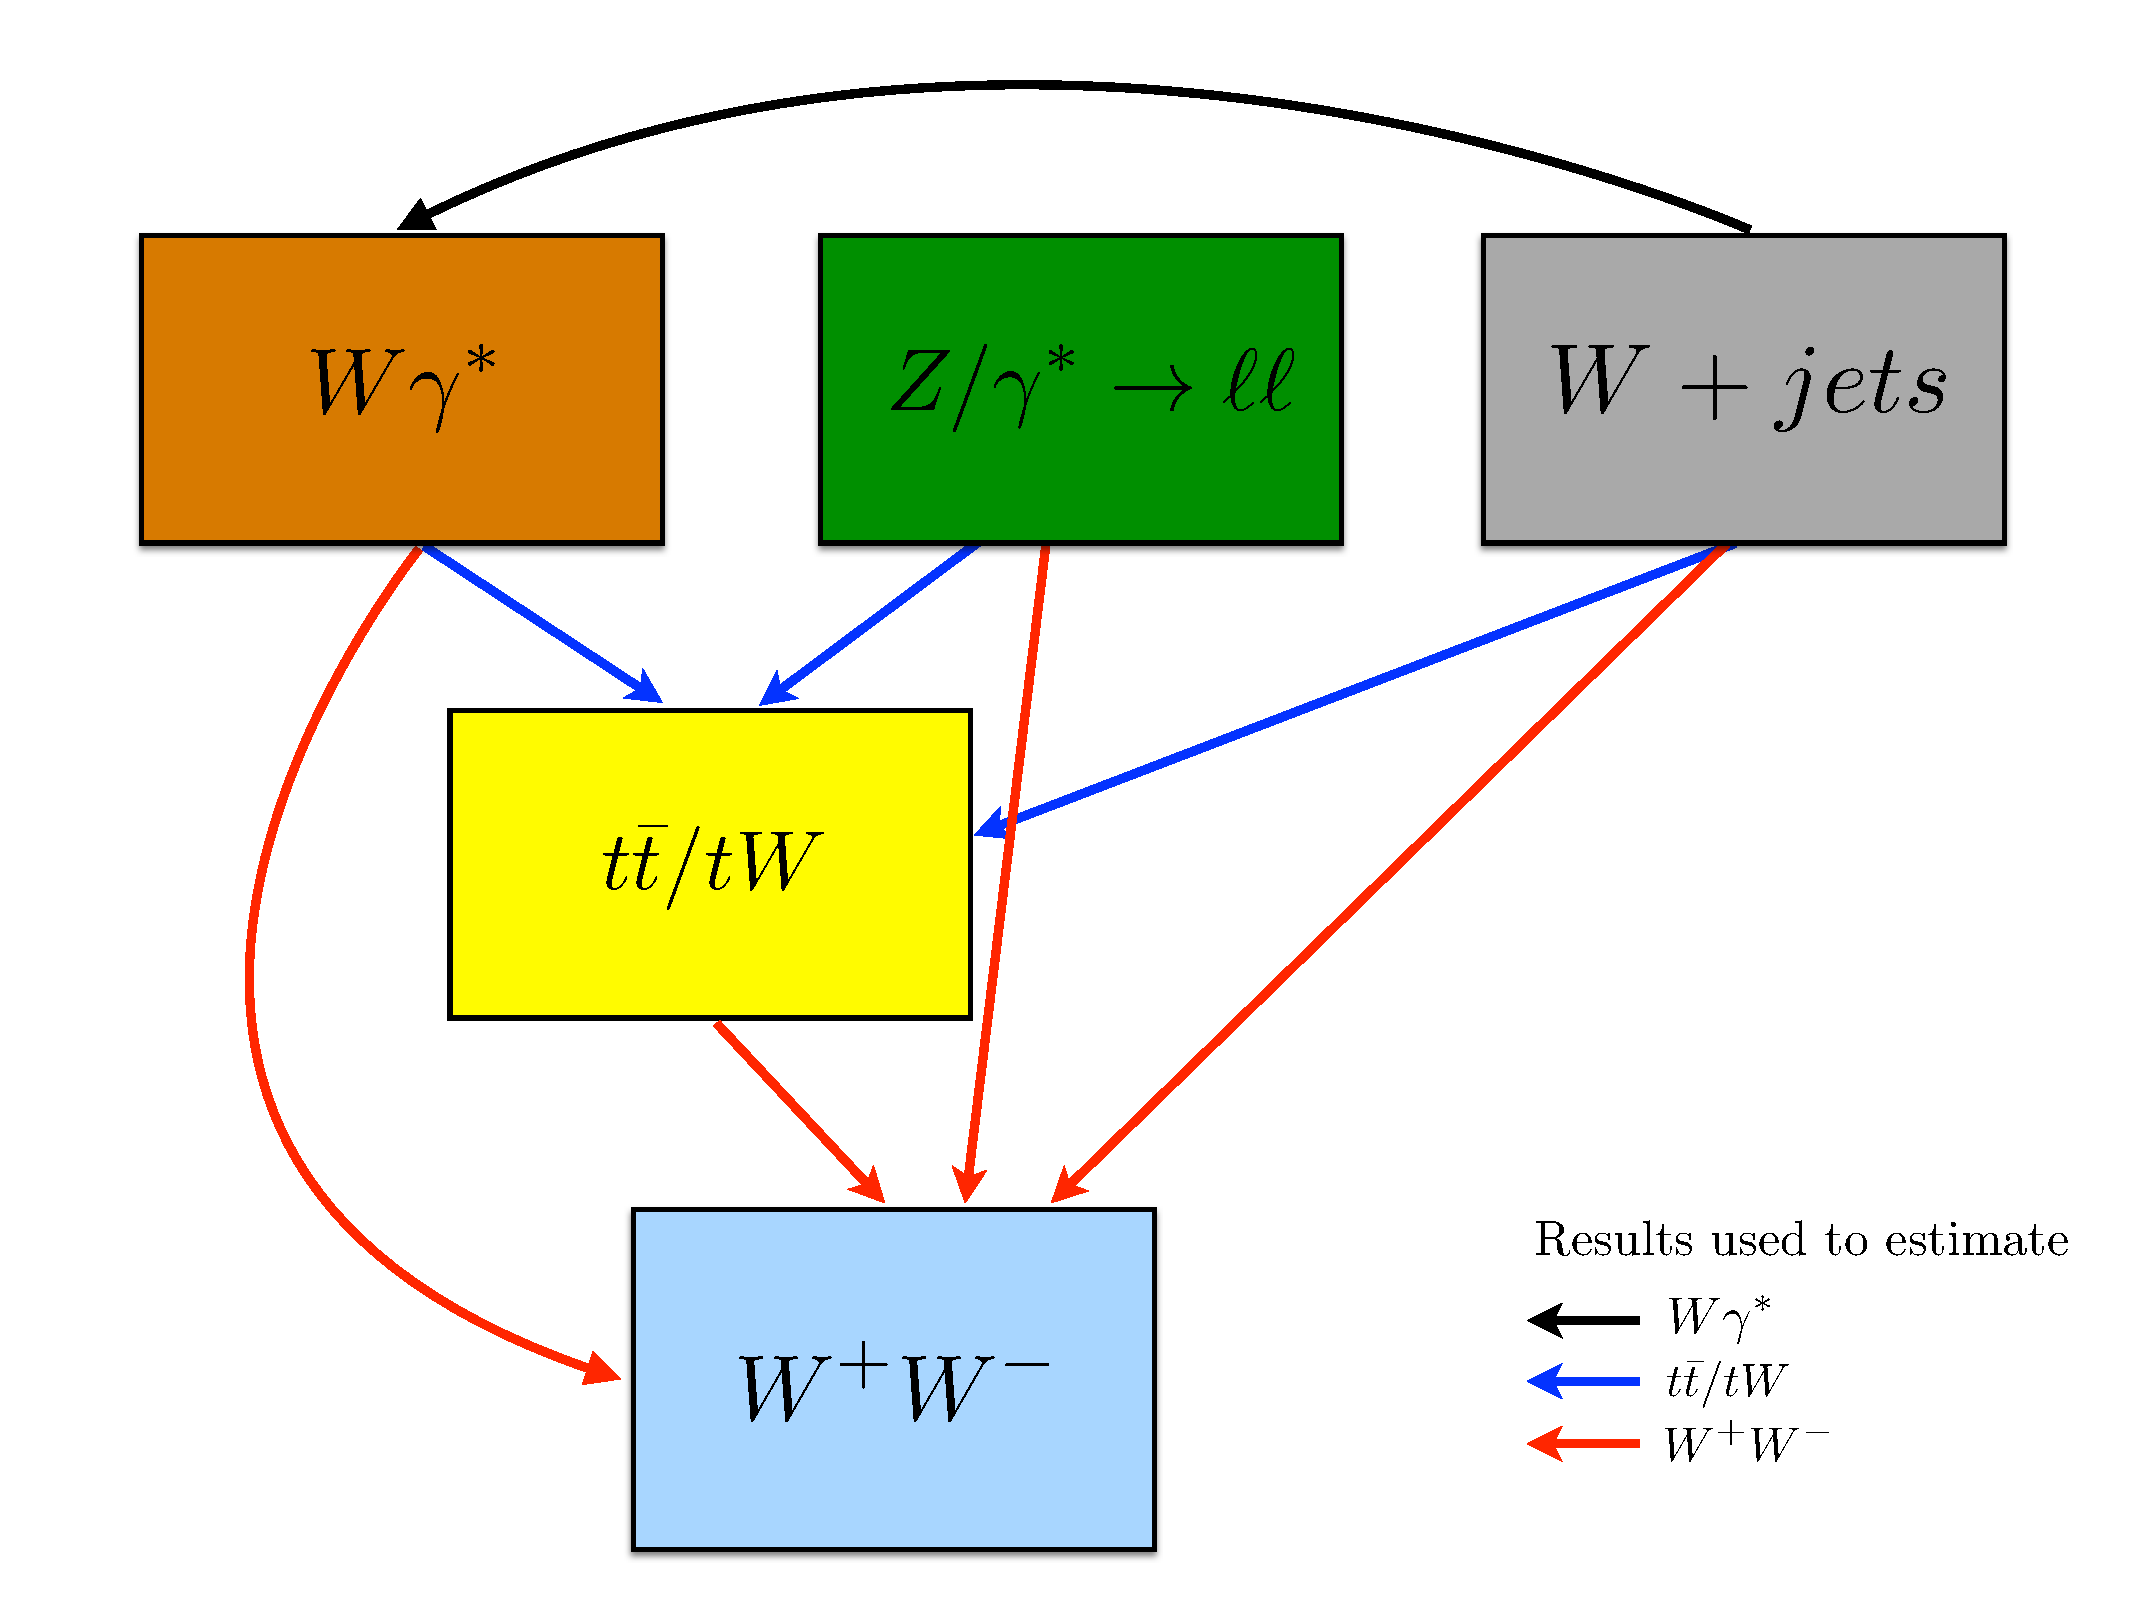
\includegraphics[width=0.99\textwidth]{figures/bkgest_schematic.pdf} 
\caption{Dependency of the data-driven estimations.} 
\label{fig:bkgest_dependency} 
\end{figure} 

%%%%%%%%%%%%%%%%%%%%%%%%%%
\section{ \dyll }

The \dyll\ is one of the main backgrounds in the \SF\ category.   
The \dyll\ events do not have intrinsic \met. But, any mis-measurements can 
lead to a fake(instrumental) \met, of which the mis-measurement of jet momentum dominates.  
The expected contribution of the \dyll\ in the signal region is estimated by 
counting events near the Z mass ($|\mll - m_Z| < 7.5~\GeV$
\footnote{Tighter mass window than Z veto requirement in the WW selection is chosen
to reduce other background contributions}) in data, subtracting 
the contributions from other processes, and scaling it by the ratio(\routin) 
which is defined as the ratio of events outside of Z peak to the events inside
of Z peak with looser BDT score. In equation, this can be written by 
\begin{eqnarray} 
N(ll)^{DY}_{SR} 
= 
%\begin{array}{ccc} \multicolumn{2}{c}{\displaystyle 
\left( N(ll)_{CR}^{data} - 0.5 \times N(e\mu)_{CR}^{data} \times k_{ll} - N_{CR}^{\vv, MC} \right) 
%} & \\ & \multicolumn{2}{c}{\hspace{8cm} \displaystyle
\times R(ll)_{out/in}
%} \end{array}   
\end{eqnarray} 
where 
\begin{itemize}
\item $ll$ : $ee$ or $\mu\mu$ 
\item $N(ll)^{DY}_{SR}$ : expected \dyll\ contribution in the signal region(SR) 
\item $N(ll)_{CR}^{data}$ : number of $ll$ data events in the control region(CR) which is 
      under the Z peak ($|\mll - m_Z| < 7.5~\GeV$)  
\item $N(e\mu)_{CR}^{data}$ : number of $e\mu$ data events in the control region(CR) which is 
      under the Z peak ($|\mll - m_Z| < 7.5~\GeV$)  
\item $k_{ll}$ : efficiency correction for $e\mu$ events,  \\
      $\displaystyle k_{ee} = \sqrt{\frac{N(ee)_{in}^{loose}}{N(\mu\mu)_{in}^{loose}}}$  and   
      $\displaystyle k_{\mu\mu} = \sqrt{\frac{N(\mu\mu)_{in}^{loose}}{N(ee)_{in}^{loose}}}$,
      measured with loose selection ($\minpmet > 20~\GeV$) 
\item $N_{CR}^{\vv, MC}$ : contribution from \vv\ events estimated in MC
\item $R(ll)_{out/in}$ : \routin\ value measured in data with looser BDT score
\end{itemize}

The number of events in the CR($N(ll)_{CR}^{data}$) is corrected by subtracting
\vv\ and $e\mu$ contribution($N(e\mu)_{CR}^{data}$) which is dominated by \topbkg, 
with an efficiency correction between \SF\ and \DF. The lepton efficiency does not depend 
on the BDT score, so we can measure it without the BDT score requirement 
to get more statistics. The statistical uncertainty on the lepton efficiency 
measured with the events under the Z peak is
much smaller($< 1~\%$) than the dominant systematic uncertainty. 
The \vv\ contribution is taken from MC because they have real \met, 
and real \met\ is well-modelled by simulation.
%\textcolor{blue}{The reason why \vv\ is considered separately from \dyll
%is that the extrapolation from CR to SR can be different for the two 
%processes once the full selection is applied.}  
For the \vv\ contribution in the CR, we assign 10 \% of systematic uncertainty.  
%\textcolor{red}{where does this 10\% come from?} 

The \routin\ is measured in data with a looser BDT score. 
The assumption is that the \routin\ does not change as a function of 
the BDT score, which is expected because the BDT score is dominantly dependent on \met,
and \met\ in \dyll\ events mostly comes from the jet momentum mis-measurement, 
which is weakly correlated to the lepton energy/momentum from which 
\mll\ is calculated. So, we divide the BDT score into 4 bins
([-0.9,-0.85], [-0.85,-0.60], [-0.60,WP], [WP,1.0]) where WP 
is 0.88 for 0-jet and 0.84 for 1-jet, and measure the 
\routin\ using the bin closest to the signal region in order to get the 
sample with similar kinematics as the signal region events.  
\begin{figure}[ht!] 
\centering 
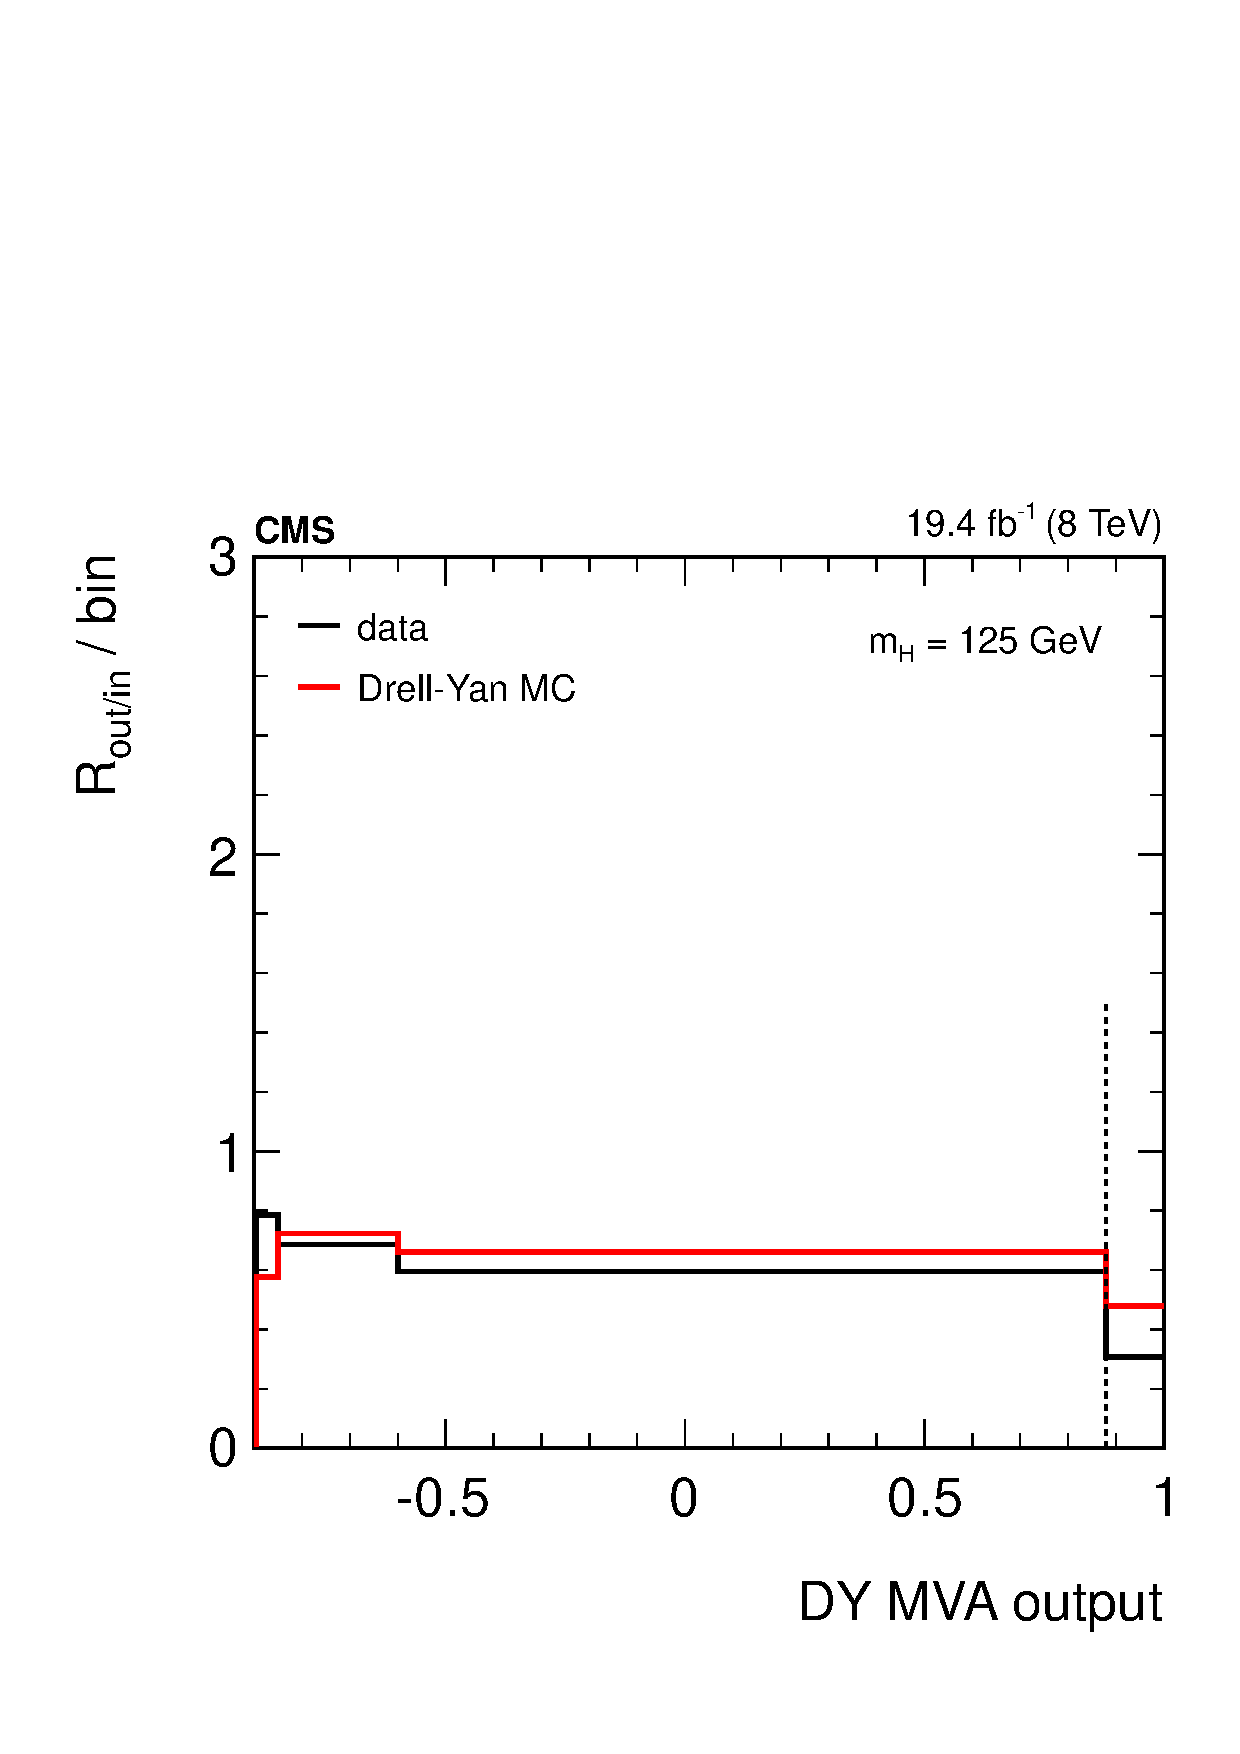
\includegraphics[width=0.5\textwidth]{figures/Routin_0Jet_mH125_19467pb_dy.pdf} 
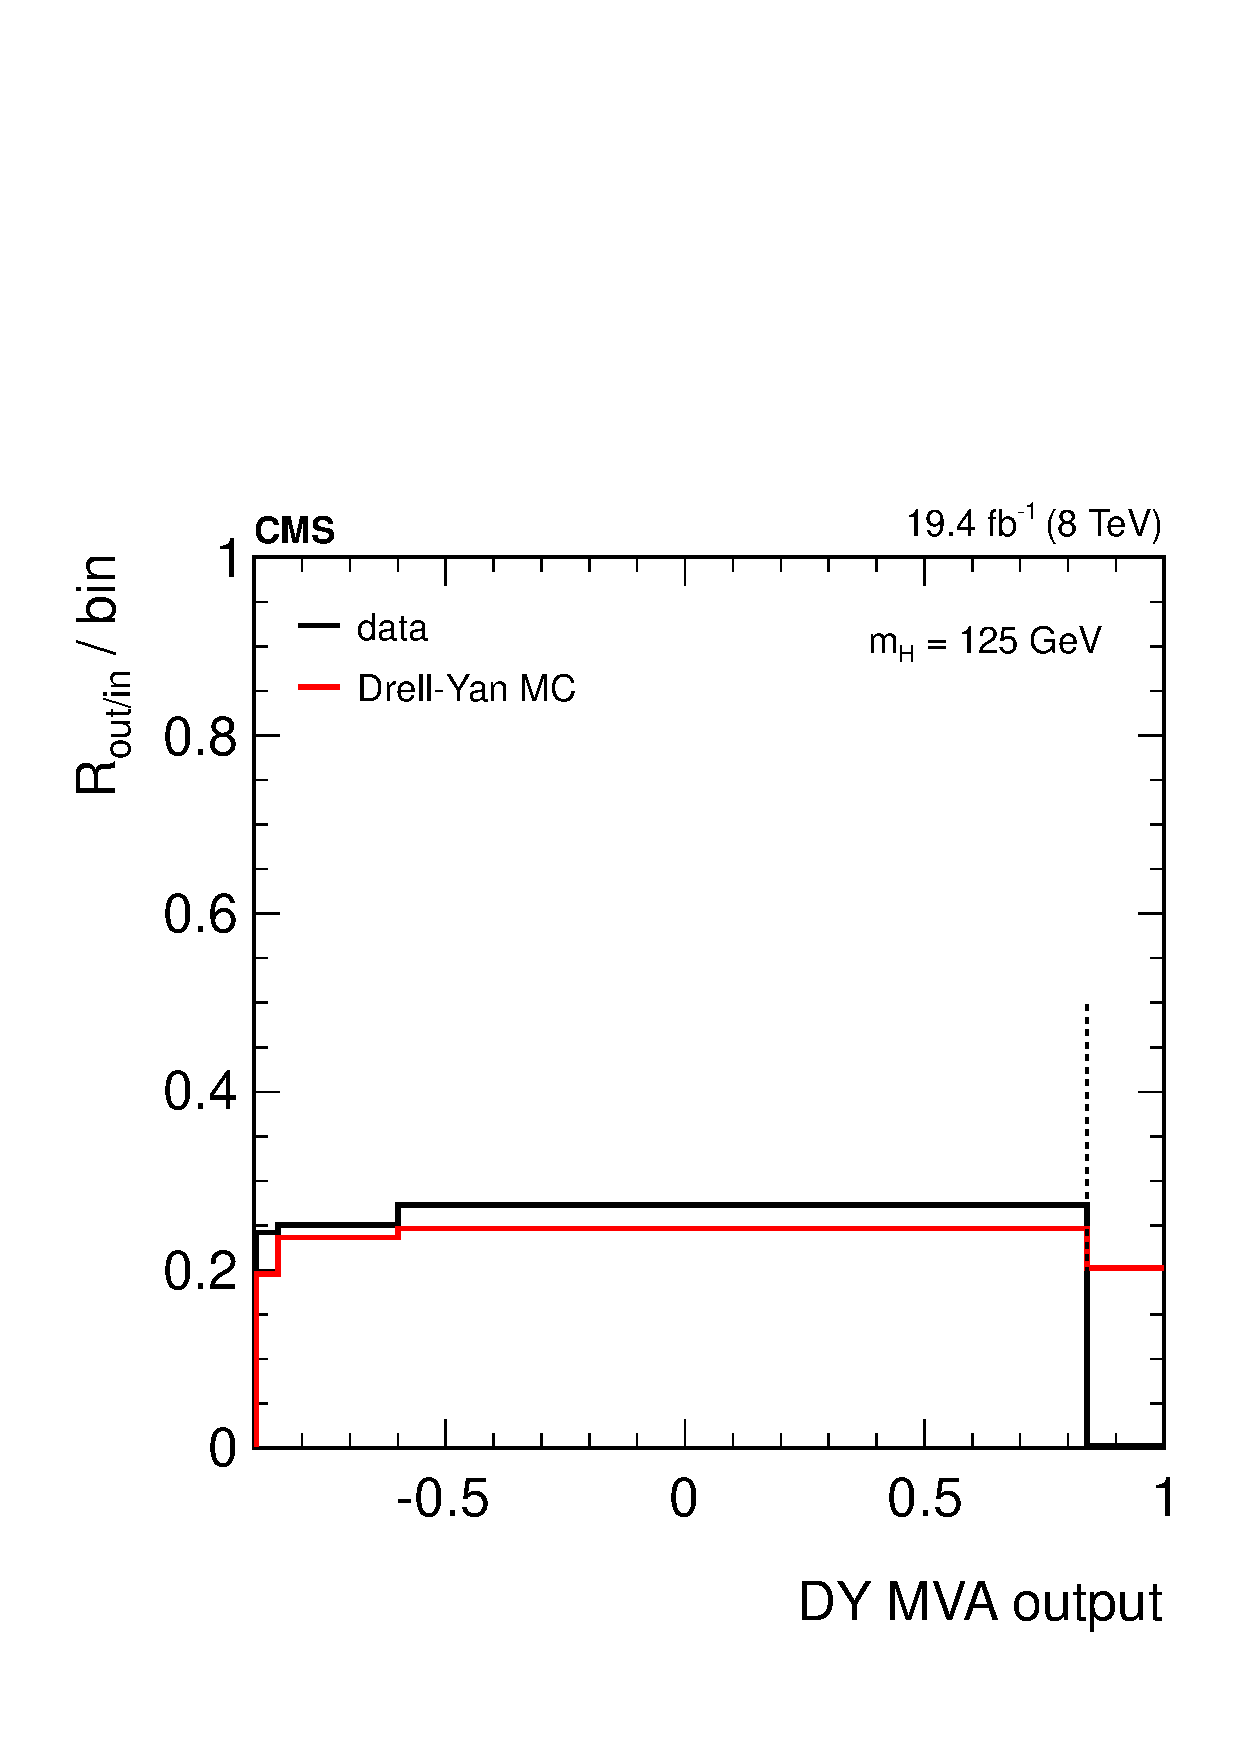
\includegraphics[width=0.5\textwidth]{figures/Routin_1Jet_mH125_19467pb_dy.pdf} 
\caption{\routin\ values as a function of BDT score for 0-jet and 1-jet categories
for \mHi=125~\GeV\ analysis. 
The black is from data subtracting \vv\ contribution and the red is from MC. 
The vertical dotted lines show the cut for signal region.} 
\label{fig:routin_mh125} 
\end{figure} 
Figure~\ref{fig:routin_mh125} shows \routin\ divided in 4 bins for 0-jet and 1-jet for 
\mHi = 125~\GeV\ analysis. The fourth bin, located after the vertical dotted lines, 
corresponds to the signal region. The results using data subtracting \vv\ component, 
and using MC are drawn as black and red, respectively. 
The results show that \routin\ is almost flat as a function of the BDT score. 

The systematic uncertainty comes from lack of ``flatness" of \routin, 
the largest difference between the third bin and the other bins.
%\textcolor{red}{how large is this?} 
In addition, there is an alternate method to estimate \dyll\ 
using the $\gamma$ + jets data sample. 
The difference between this method and \routin\ method in 
the extrapolation from CR to SR is about 30\%. 
We take the maximum of the lack of flatness and the 30~\% 
as the final systematics of the estimation. 

At the end we merge $ee$ and $\mu\mu$ to get more statistics. 
The table~\ref{tab:dy_wwlevel} shows the final estimation at WW level.
The table~\ref{tab:dy} shows the final estimation of \dyll\ at all 
\mHi\ hypotheses up to 300 \GeV. 
After 300 \GeV, the $N_{out}(data)/N_{out}(MC)$ scale factor for WW selection 
is applied. 

%%%%%%%%%%%%%%%%%%%%%%%%%%%%%% 
\begin{table}
\begin{center}
\small
\vspace{0.5cm}
\caption{The Drell-Yan estimation in the same flavor final state at WW selection level.}
\vspace{0.5cm}
\label{tab:dy_wwlevel}
\begin{tabular}{c c c c c c}
\hline
       $N_{jet}$ & $N_{in}$(data)        & $R_{out/in}$        & $N_{out}$(data)  & $N_{out}$ (MC) \\ 
\hline
0 & $775.16\pm74.47$ & $0.28\pm0.01\pm0.08$ & $218.64\pm21.53\pm65.59$ & $34.64\pm9.56$ \\
1 & $350.69\pm38.00$ & $0.25\pm0.01\pm0.08$ & $89.20\pm9.83\pm26.76$ & $21.05\pm7.16$ \\
\hline
\end{tabular}
\end{center}
\end{table}

%%%%%%%%%%%%%%%%%%%%%%%%%%%%%%
\begin{table}
\begin{center}
\footnotesize
\vspace{0.5cm} 
\caption{The Drell-Yan estimation in \DF\ channel for the cut-based selections.
The dependence of \routin\ on \mHi\ is due to the \mHi-dependent selection listed in 
Table~\ref{tab:cutbasedtable}.}
\vspace{0.5cm} 
\label{tab:dy}
\begin{tabular}{c c c c c c}
\hline
\hline
\multicolumn{5}{c}{0-jet} \\
\hline
mass & $N_{in}$(data)        & $R_{out/in}$        & $N_{out}$(data)  & $N_{out}$ (MC) \\ 
\hline
%\vspace{-3mm}  \\
115 \GeV & $145.94\pm15.08$ & $0.31\pm0.01\pm0.09$ & $45.07\pm4.81\pm13.52$ & $8.70\pm5.08$ \\
120 \GeV & $263.31\pm20.83$ & $0.31\pm0.01\pm0.09$ & $81.33\pm6.80\pm24.40$ & $13.57\pm5.88$ \\
125 \GeV & $154.60\pm16.13$ & $0.60\pm0.02\pm0.19$ & $92.22\pm9.98\pm29.33$ & $16.64\pm6.63$ \\
130 \GeV & $119.10\pm14.17$ & $0.87\pm0.03\pm0.26$ & $103.61\pm12.74\pm31.08$ & $16.64\pm6.63$ \\
135 \GeV & $112.30\pm14.57$ & $0.83\pm0.03\pm0.25$ & $93.52\pm12.49\pm28.06$ & $14.53\pm6.29$ \\
140 \GeV & $108.72\pm14.48$ & $0.74\pm0.02\pm0.22$ & $80.72\pm11.09\pm24.22$ & $17.17\pm6.82$ \\
150 \GeV & $91.78\pm14.57$ & $0.40\pm0.02\pm0.12$ & $37.01\pm6.20\pm11.10$ & $7.60\pm4.47$ \\
160 \GeV & $21.03\pm8.64$ & $0.90\pm0.06\pm0.27$ & $18.83\pm7.85\pm5.65$ & $7.60\pm4.47$ \\
170 \GeV & $9.70\pm8.14$ & $0.82\pm0.06\pm0.25$ & $7.92\pm6.68\pm2.38$ & $7.60\pm4.47$ \\
180 \GeV & $7.06\pm9.35$ & $0.62\pm0.05\pm0.19$ & $4.34\pm5.76\pm1.34$ & $5.71\pm4.05$ \\
190 \GeV & $64.23\pm15.78$ & $0.34\pm0.02\pm0.10$ & $21.63\pm5.51\pm6.49$ & $10.31\pm5.20$ \\
200 \GeV & $94.35\pm21.88$ & $0.21\pm0.01\pm0.06$ & $20.10\pm4.83\pm6.03$ & $7.67\pm4.47$ \\
250 \GeV & $193.85\pm36.84$ & $0.06\pm0.00\pm0.02$ & $11.17\pm2.24\pm3.35$ & $7.08\pm4.09$ \\
300 \GeV & $89.23\pm27.97$ & $0.13\pm0.01\pm0.04$ & $11.16\pm3.62\pm3.35$ & $7.08\pm4.09$ \\
\hline
\hline
\multicolumn{5}{c}{1-jet} \\
\hline
mass & $N_{in}$(data)        & $R_{out/in}$        & $N_{out}$(data)  & $N_{out}$ (MC) \\ 
\hline
%\vspace{-3mm}  \\
115 \GeV & $28.00\pm8.66$ & $0.19\pm0.00\pm0.06$ & $5.28\pm1.64\pm1.58$ & $2.16\pm2.16$ \\
120 \GeV & $71.36\pm12.41$ & $0.19\pm0.00\pm0.06$ & $13.45\pm2.36\pm4.04$ & $4.35\pm3.08$ \\
125 \GeV & $53.67\pm10.57$ & $0.27\pm0.01\pm0.08$ & $14.69\pm2.92\pm4.41$ & $4.35\pm3.08$ \\
130 \GeV & $39.38\pm9.49$ & $0.36\pm0.01\pm0.11$ & $14.21\pm3.44\pm4.26$ & $4.35\pm3.08$ \\
135 \GeV & $45.07\pm9.97$ & $0.34\pm0.01\pm0.10$ & $15.32\pm3.41\pm4.60$ & $4.35\pm3.08$ \\
140 \GeV & $46.46\pm10.18$ & $0.31\pm0.01\pm0.09$ & $14.32\pm3.16\pm4.30$ & $4.35\pm3.08$ \\
150 \GeV & $59.54\pm12.09$ & $0.20\pm0.01\pm0.06$ & $11.79\pm2.43\pm3.54$ & $2.19\pm2.19$ \\
160 \GeV & $20.90\pm6.94$ & $0.42\pm0.02\pm0.13$ & $8.80\pm2.95\pm2.64$ & $0.00\pm0.00$ \\
170 \GeV & $16.48\pm6.89$ & $0.39\pm0.02\pm0.12$ & $6.49\pm2.73\pm1.95$ & $0.00\pm0.00$ \\
180 \GeV & $22.86\pm8.18$ & $0.33\pm0.01\pm0.10$ & $7.51\pm2.71\pm2.25$ & $0.00\pm0.00$ \\
190 \GeV & $70.87\pm13.43$ & $0.22\pm0.01\pm0.07$ & $15.71\pm3.04\pm4.71$ & $0.00\pm0.00$ \\
200 \GeV & $99.31\pm16.50$ & $0.17\pm0.01\pm0.05$ & $16.60\pm2.83\pm4.98$ & $0.00\pm0.00$ \\
250 \GeV & $128.66\pm21.79$ & $0.09\pm0.00\pm0.03$ & $12.08\pm2.11\pm3.63$ & $2.65\pm2.65$ \\
300 \GeV & $71.21\pm17.81$ & $0.11\pm0.01\pm0.03$ & $7.94\pm2.03\pm2.38$ & $5.00\pm3.54$ \\
\hline
\end{tabular}
\end{center}
\end{table}



%%%%%%%%%%%%%%%%%%%%%%%%%%
\section{ Jet-induced backgrounds : \Wjets} 
\label{sec:wjets}

As discussed in chapter~\ref{ch:event_selection}, 
jets can fake leptons(electron or muon) in various ways, 
as a result, \Wjets\ is the second largest background in the most 
sensitive channel, 0-jet \DF. 
Most of the jet-induced background comes from \Wjets\ where one jet fakes a lepton(single fake)
and a small contribution comes from QCD events where two jets fake two leptons(double fakes).  
Even though the cross section of QCD process is huge, the probability for a jet 
to fake a lepton is very small, being in the order of 
$\mathcal{O}(10^{-3}) \sim \mathcal{O}(10^{-5})$
depending on the kinematics. In addition, QCD events do not have a source of true \met\, 
so the contribution is suppressed dramatically by the tight \met\ requirement. 
In the end, the contribution of the double fakes is negligible compared to the 
systematic uncertainty of the method, so it is not explicitly taken into account in this analysis. 

The estimation of the jet-induced background starts from measuring the ``fake rate(FR)"
that is defined as the probability for a lepton with loose selection to pass the full selection. 
The leptons that pass the loose selection are called ``fakable object(FO)". The fake rate is 
measured in the data events that is dominated by QCD di-jet events collected 
by pre-scaled low \pt\ single-lepton triggers. 
The measured FR is applied to the data sample where the lepton selection 
of one of the leptons is loosened. 
The details will be discussed in the following subsections.

\subsubsection{Definition of fakable objects}

The definition of FO is limited by the analysis triggers used to collect the signal events. 
We can not define FO to be looser than the trigger requirement because FR can be 
biased due to tighter FO selection caused by the trigger requirement. Therefore, the 
loosest selection that we can afford is the trigger requirement. For electron,  
we use the following definition which is basically an offline version of the trigger selection
with conversion rejection added : 
\begin{itemize}
  \item $\pt>10~\GeV$ and $|\eta| < 2.5$
  \item $\sigma_{i\eta i\eta} < 0.01/0.03$ (barrel/endcap)
  \item $|\Delta\phi_{in}| < 0.15/0.10$ (barrel/endcap)
  \item $|\Delta\eta_{in}| < 0.007/0.009$ (barrel/endcap)
  \item $\textrm{H/E}< 0.12/0.10$ (barrel/endcap)
  \item $\displaystyle \frac{\sum_{\textrm{tracks with dR}<0.3}\Et}{\pt}<0.2$
  \item $\displaystyle \frac{\left(\sum_{\textrm{ECAL with dR}<0.3}\Et\right)-1}{\pt}<0.2$
  \item $\displaystyle \frac{\sum_{\textrm{HCAL with dR}<0.3}\Et}{\pt}<0.2$
  \item conversion rejection 
\end{itemize}
The background caused by photon conversions 
can have different FR, so it is not estimated by this method. 
By excluding the contribution from the conversion rejection, 
we construct a sample of FO with similar sources. 

The definition of muon FO is given by relaxing the transverse impact parameter and 
the isolation requirements :  
\begin{itemize}
    \item $\left|d_0\right| < 0.2$~cm
    \item Isolation MVA output $>$ -0.6
\end{itemize}
The definition for muon is simpler because of the loose trigger requirement. 

\subsubsection{Measurement of fake rate}

The FR is measured in data dominated by QCD di-jet events. 
These events are collected by single-lepton triggers listed in Table~\ref{tab:triggers_util}.
The events selected by these triggers are dominated by leptons that 
originate from quarks and gluons. 

Though the sample is dominated by QCD 
events, there are contributions from Electroweak(EWK) processes such as \Wjets\ and \dyll. 
In order to suppress \Wjets\ contribution, $\met>20~\GeV$ and $\mT<15~\GeV$ are required. 
The residual contribution is estimated using simulation normalized by a data/MC scale factor 
calculated using the bulk of \Wjets\ events defined as $\met>30~\GeV$, $60<\mT<90~\GeV$ 
and the full lepton selection. The deviation of scale factor from unity 
is taken as a systematic uncertainty for FR measurement due to the \Wjets\ contribution.
%The scale factor is 0.81 and 1.06 in the muon and electron
The \dyll\ contribution is suppressed by rejecting events 
that contain an additional lepton that makes an opposite-sign lepton pair 
with di-lepton mass within 15~\GeV\ of the Z mass.  
The residual contribution is estimated using simulation normalized by a data/MC scale factor
calculated using events within 15~\GeV\ of the Z mass.
The deviation of scale factors from unity
is taken as a systematic uncertainty for FR measurement due to the \dyll\ contribution .
%The scale factor is 1.15 and 0.94 for the muon and electron

Another EWK contribution comes from di-electron events when the second electron 
is outside of the tracker acceptance. This electron is not reconstructed 
as an electron because it does not have a track, but can be reconstructed 
as a jet. The result is an event with one lepton and low \met, which 
can fall into the FO selection. In order to suppress this, the $\left| \eta \right|$ 
of the jet that recoils against FO is required to be less than 2.5. For di-muon events 
this does not happen because if a muon is outside of tracker acceptance, 
it is not reconstructed as muon, giving a large \met\ in the event. 
This event is not selected for FO because of high \met. 

\begin{figure}[htp] 
\centering 
\begin{tabular}{c} 
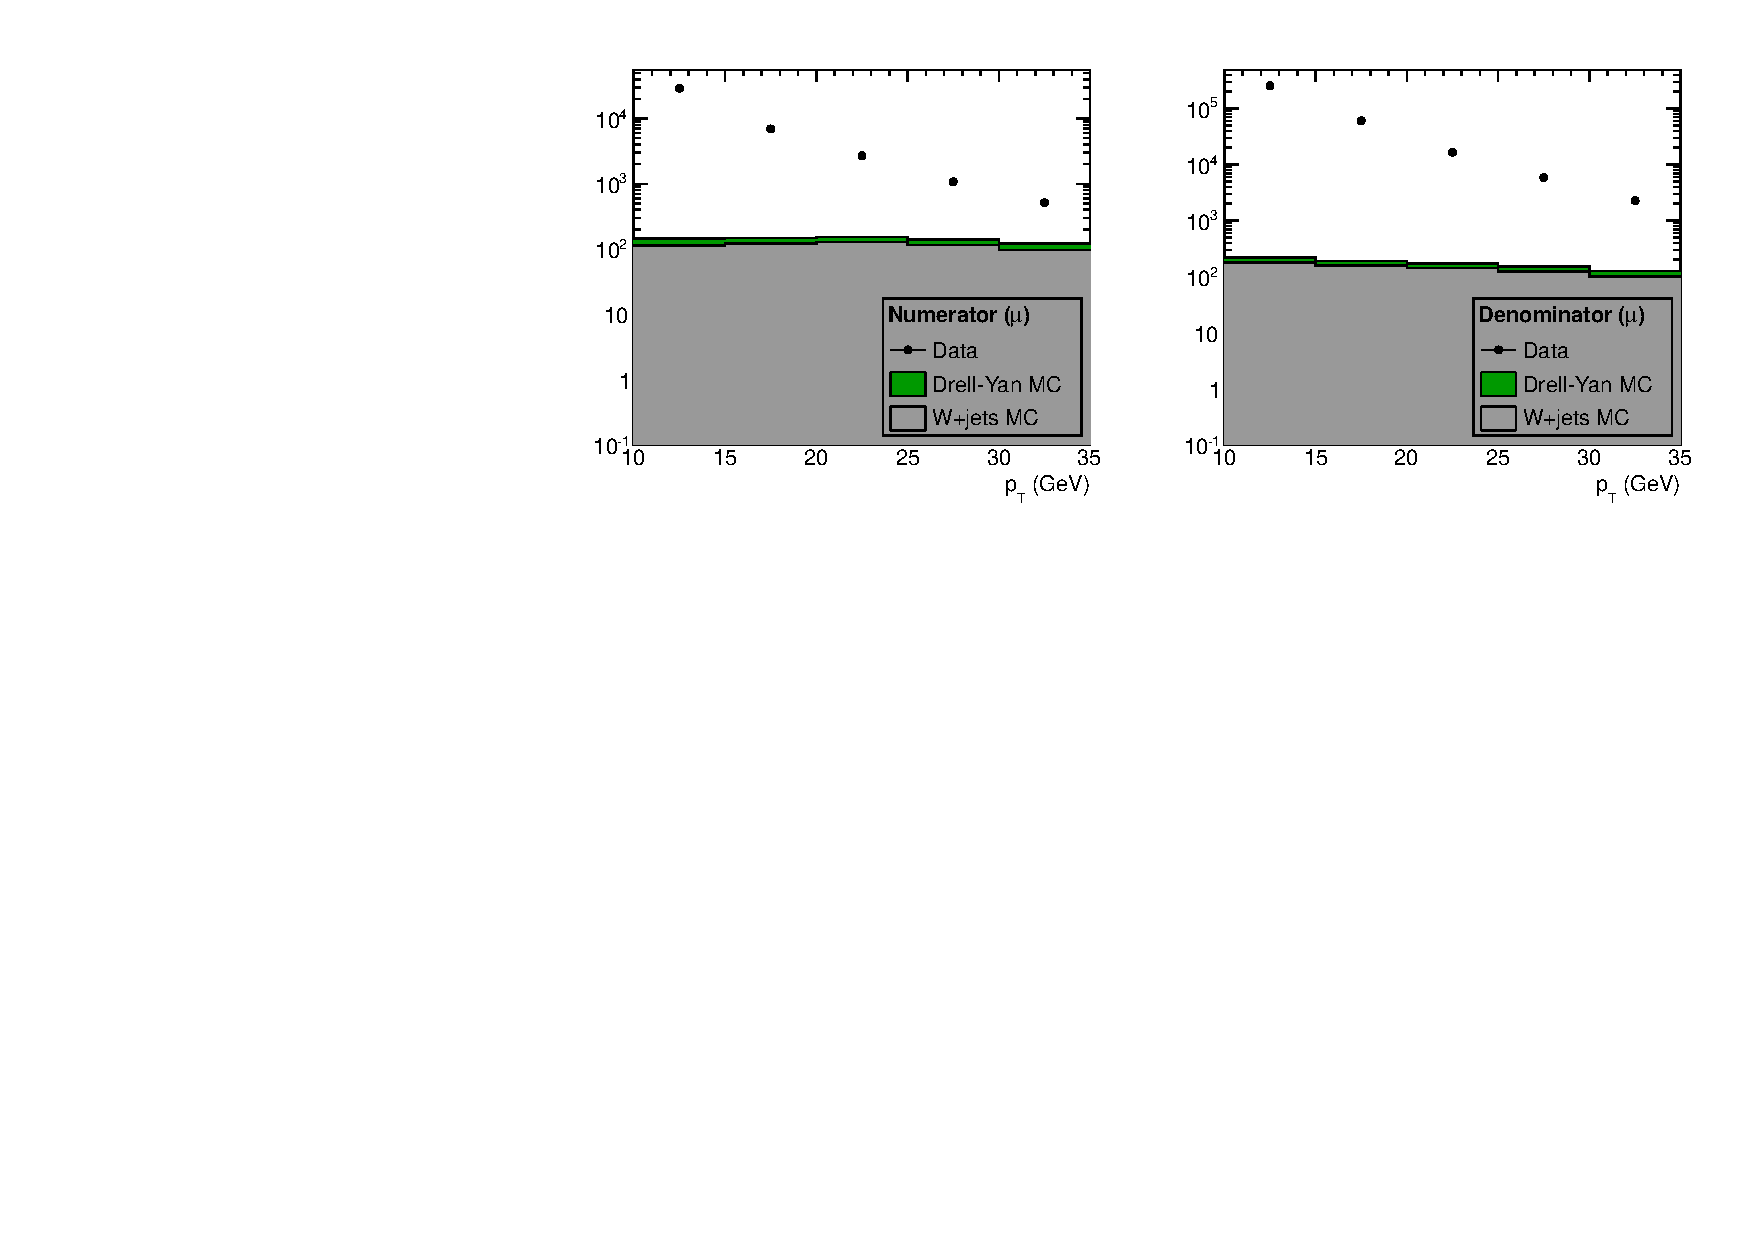
\includegraphics[width=1.00\textwidth]{figures/Num_den_pt_Mu.pdf}  \\
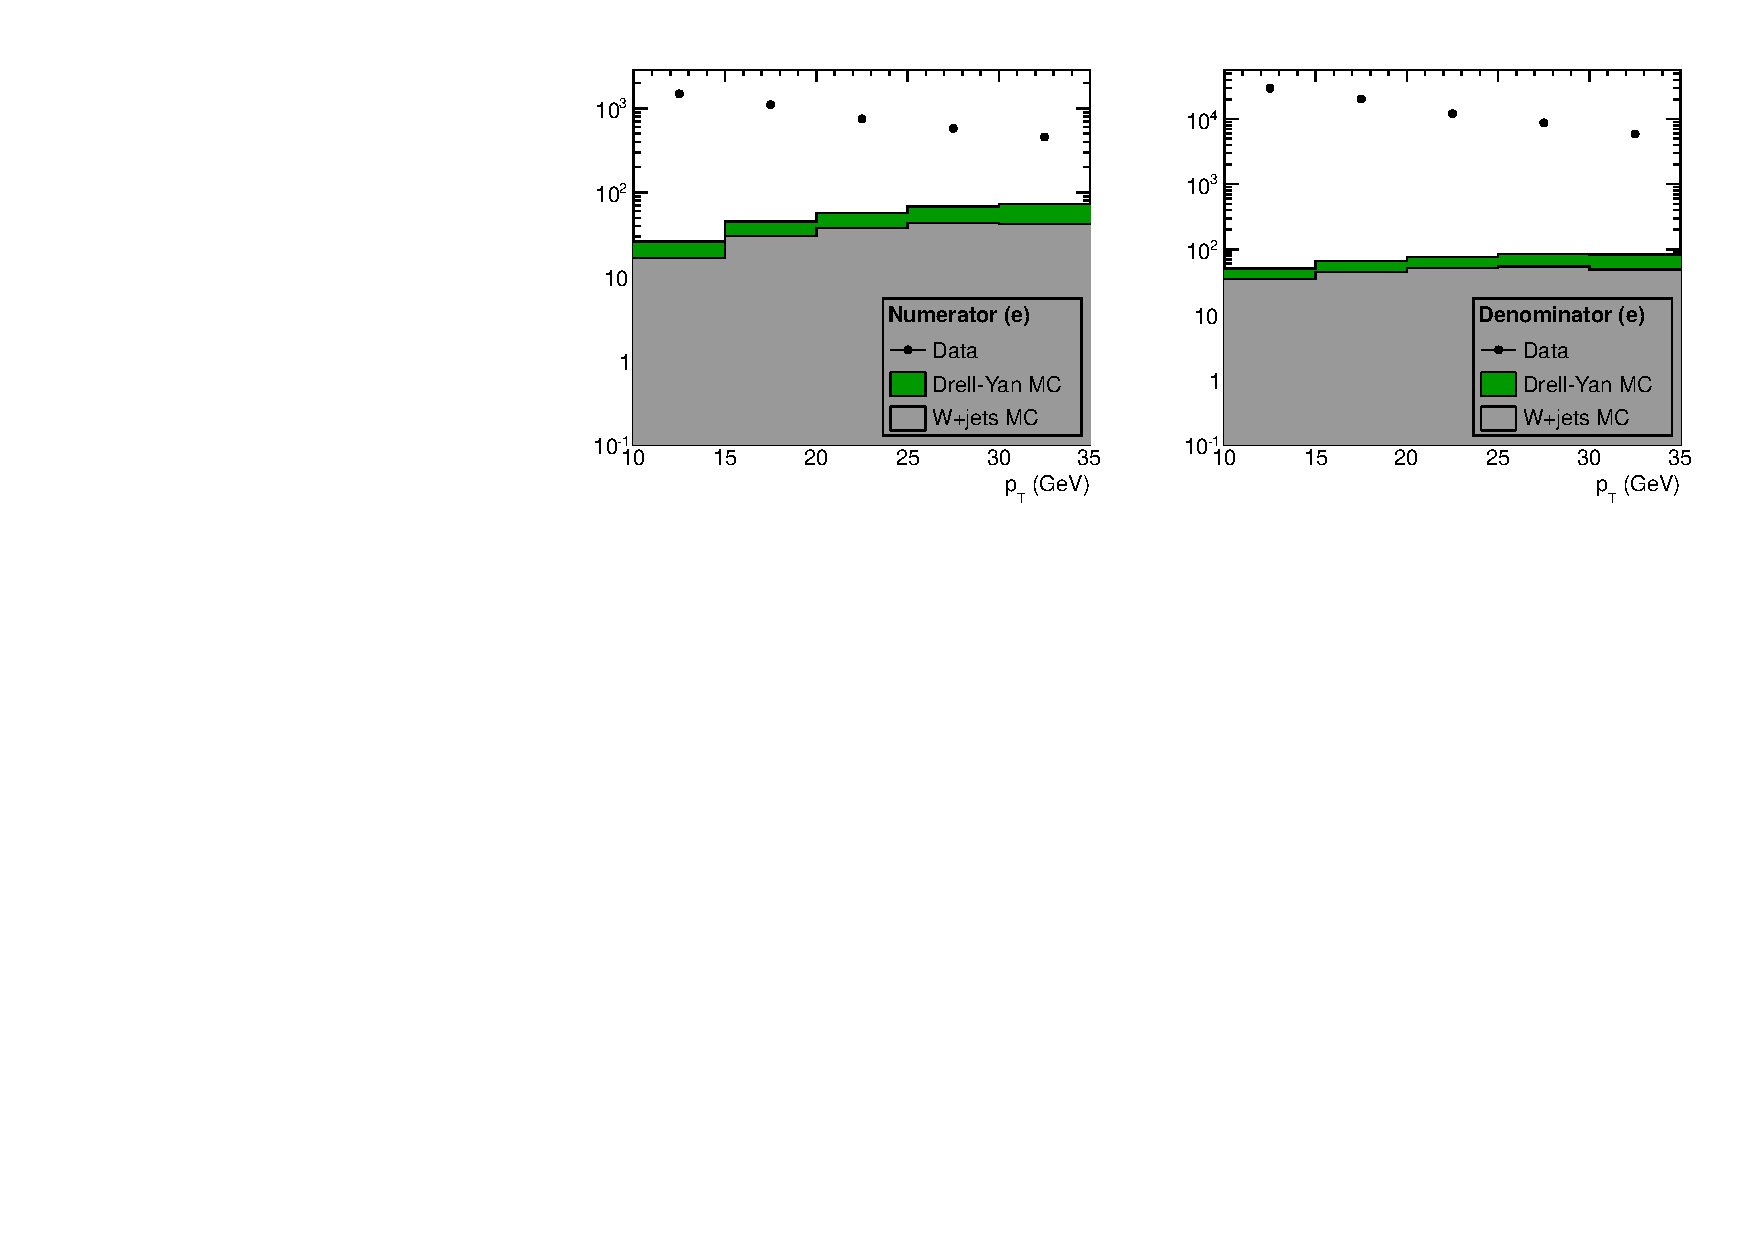
\includegraphics[width=1.00\textwidth]{figures/Num_den_pt_Ele.pdf}
\end{tabular} 
\caption{The \pt\ of denominator(left) and numerator(right) of 
muon FO(top) and electron FO(bottom). The black dots represent 
data and solid histograms represent contributions from Drell-Yan(green) 
and W+jets(grey). It is obvious 
that the contribution from EWK processes is quite large at high FO \pt\ 
and FR would be higher if EWK contribution were not subtracted
because FR of EWK sample is higher than the FR of QCD di-jet sample.  }
\label{fig:Num_Den_pt_EWK} 
\end{figure} 

Figure~\ref{fig:Num_Den_pt_EWK} shows the \pt\ distributions of the denominator and the 
numerator of electron and muon FO. The data is shown with black dots and 
the EWK contributions from \dyll\ and \Wjets\ are shown in green 
and grey, respectively. At higher \pt\ the relative EWK contribution 
is larger. Because FR is higher in \Wjets\ events than the QCD di-jet 
events, if EWK contribution were not subtracted, the FR would be 
measured higher than it should be. The subtraction of the EWK contribution 
reduces FR in the last \pt\ bins by up to 30 \%.

A fake lepton originates from a parton, and the fake rates have strong 
correlation with the \pt\ of the parton from which a fake lepton originates.
So, it is very important to use similar kinematic region when measuring FR 
with that of the region where the FR is applied. The best handle to select 
a relevant kinematic region is the 
\pt\ of the progenitor parton, but this information is not available in data.   
So, we use the \pt\ of the jet which is separated by $\Delta \textrm{R(FO, leading jet)} > 1.0$
as an approximate handle of the progenitor \pt. This jet is called ``away jet".  
Given that the FR is measured with the sample dominated by QCD di-jet events, 
the FO and the leading jet tend to be back-to-back in the $r-\phi$ plane.
Therefore, by gauging the \pt\ of the away jet, we can gauge the \pt\ 
of the progenitor of the FO. Ideally this works, but reality is more 
complicated because the \pt\ of the away jet does not necessarily represent 
the \pt\ of the progenitor of the FO. The away jet \pt\ can be mis-measured 
and the direction of the jet can be off back-to-back direction.  
Therefore, it is not straightforward to decide the \pt\ of the away jet. 

We use same-sign events to make sure that we select the 
relevant kinematic range of the progenitor for the \Wjets\ sample. 
These events are dominated by \Wjets\ and $\wgamma(^*)$. 
Since we can control $\wgamma(^*)$
relatively well, we can use these events to confirm that the measured 
FR predicts the data correctly. 
But, even though the prediction is consistent with observation, 
we can not conclusively claim that the measured FR is correct 
because the composition of the fakes can be different in the same-sign 
and the opposite-sign events. 
For example, same-sign events can not originate from W+q events, 
which result in an opposite-sign lepton pair\footnote{If W has (+1) charge, 
q has (-1/3) charge which makes up a (-1) charge meson, and it subsequently decays 
to a (-) charge lepton. The ratio of the opposite-sign to the same-sign events 
measured in \Wjets\ MC is 6:4}. Therefore, the result using the same-sign events can 
give a rough idea, but we can not conclusively decide the away jet \pt from them. 

The away jet \pt\ thresholds are determined based on multiple information.  
The first information is the comparison in simulation 
of the \pt\ spectrum of the jets in the \Wjets\ 
sample and the jets in the QCD sample that envelop the FO. The other information 
is the comparison of the isolation variable of FO in the QCD events and the \Wjets\ 
events in data. These show that the best match is attained when  
using 35~\GeV\ for electrons and 30~\GeV\ for muons. 
Figure~\ref{fig:2DFR} shows the FR for muons and electrons using these thresholds. 
The expected same-sign events in the 0-jet category  
is $794\pm18(stat.)$ while the number of observed data events is 752 which 
is consistent with the expectation.
\begin{figure}[htp] 
\centering 
\begin{tabular}{c} 
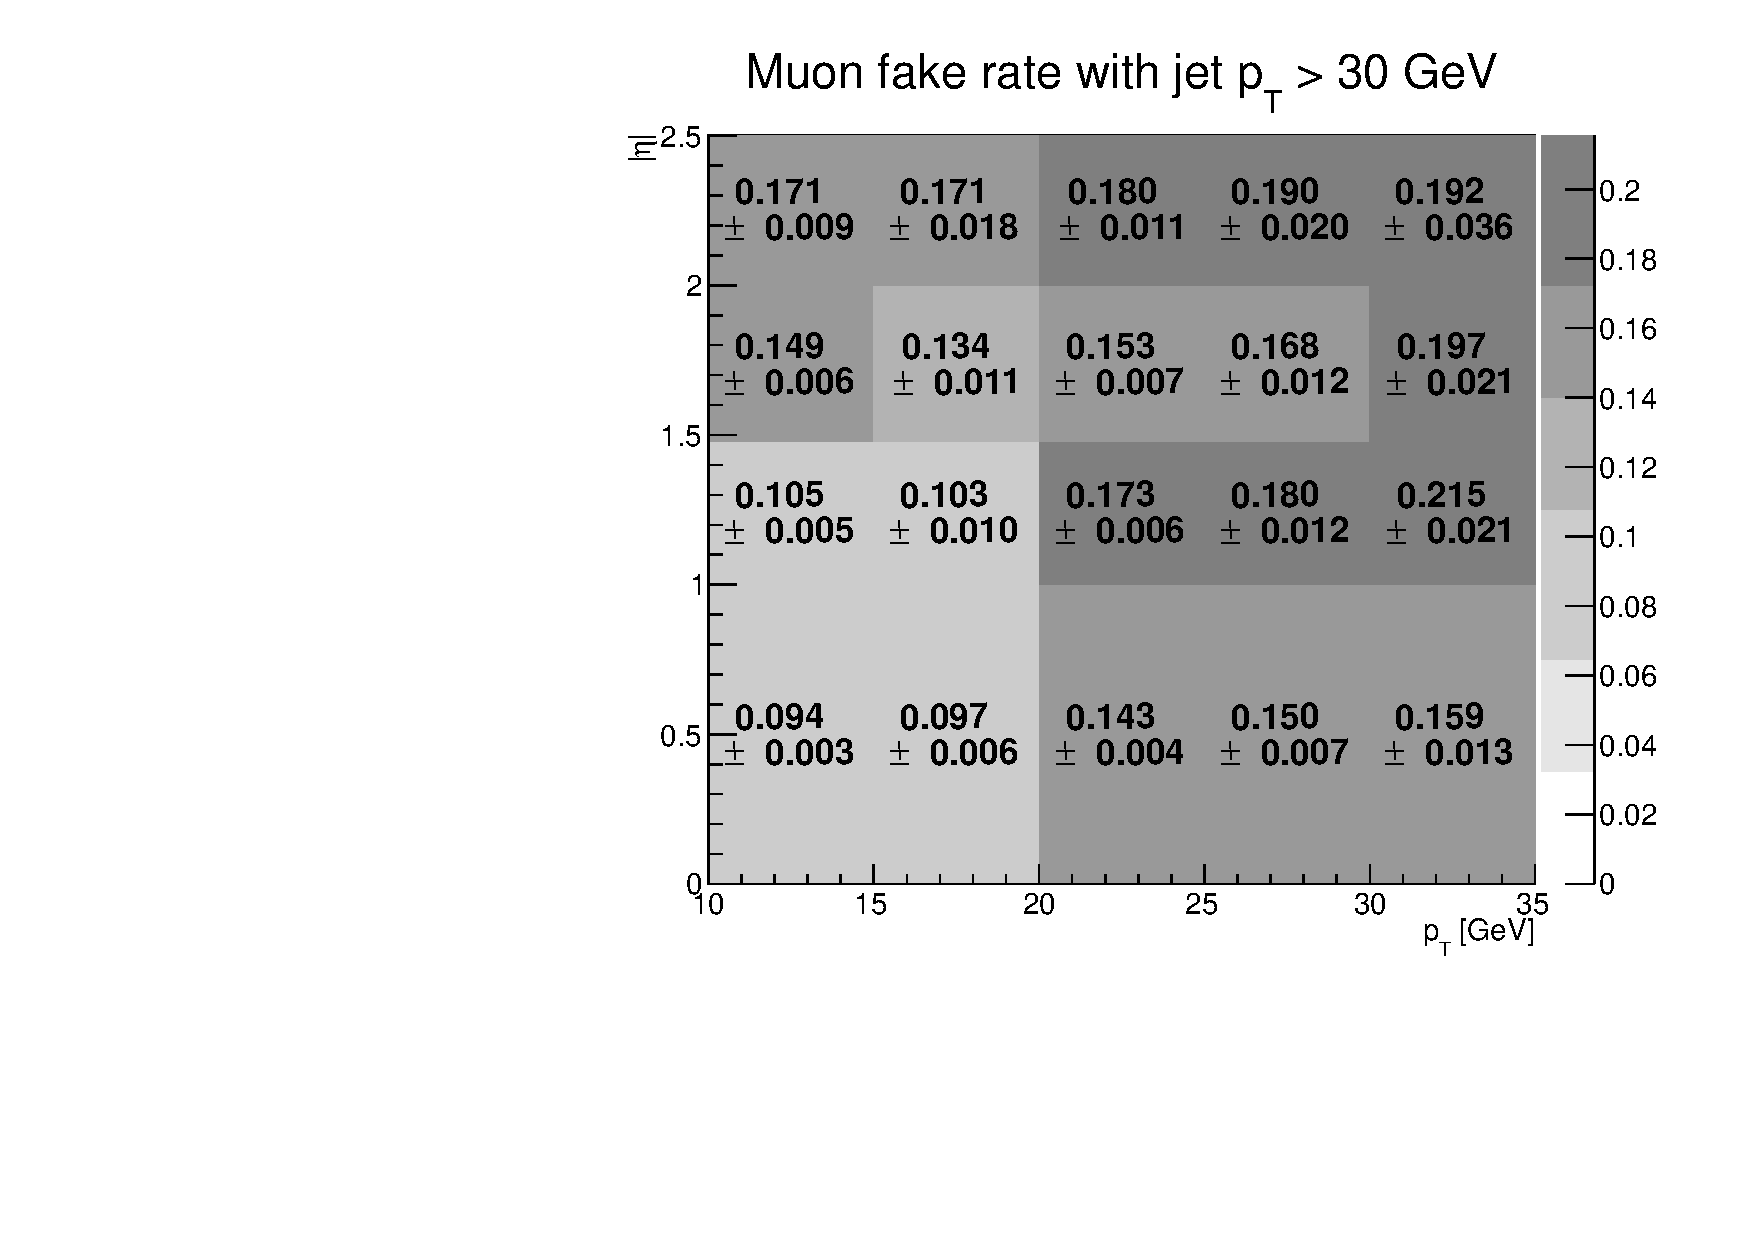
\includegraphics[width=0.75\textwidth]{figures/2DFR_Muon_jet30.pdf} \\
\\
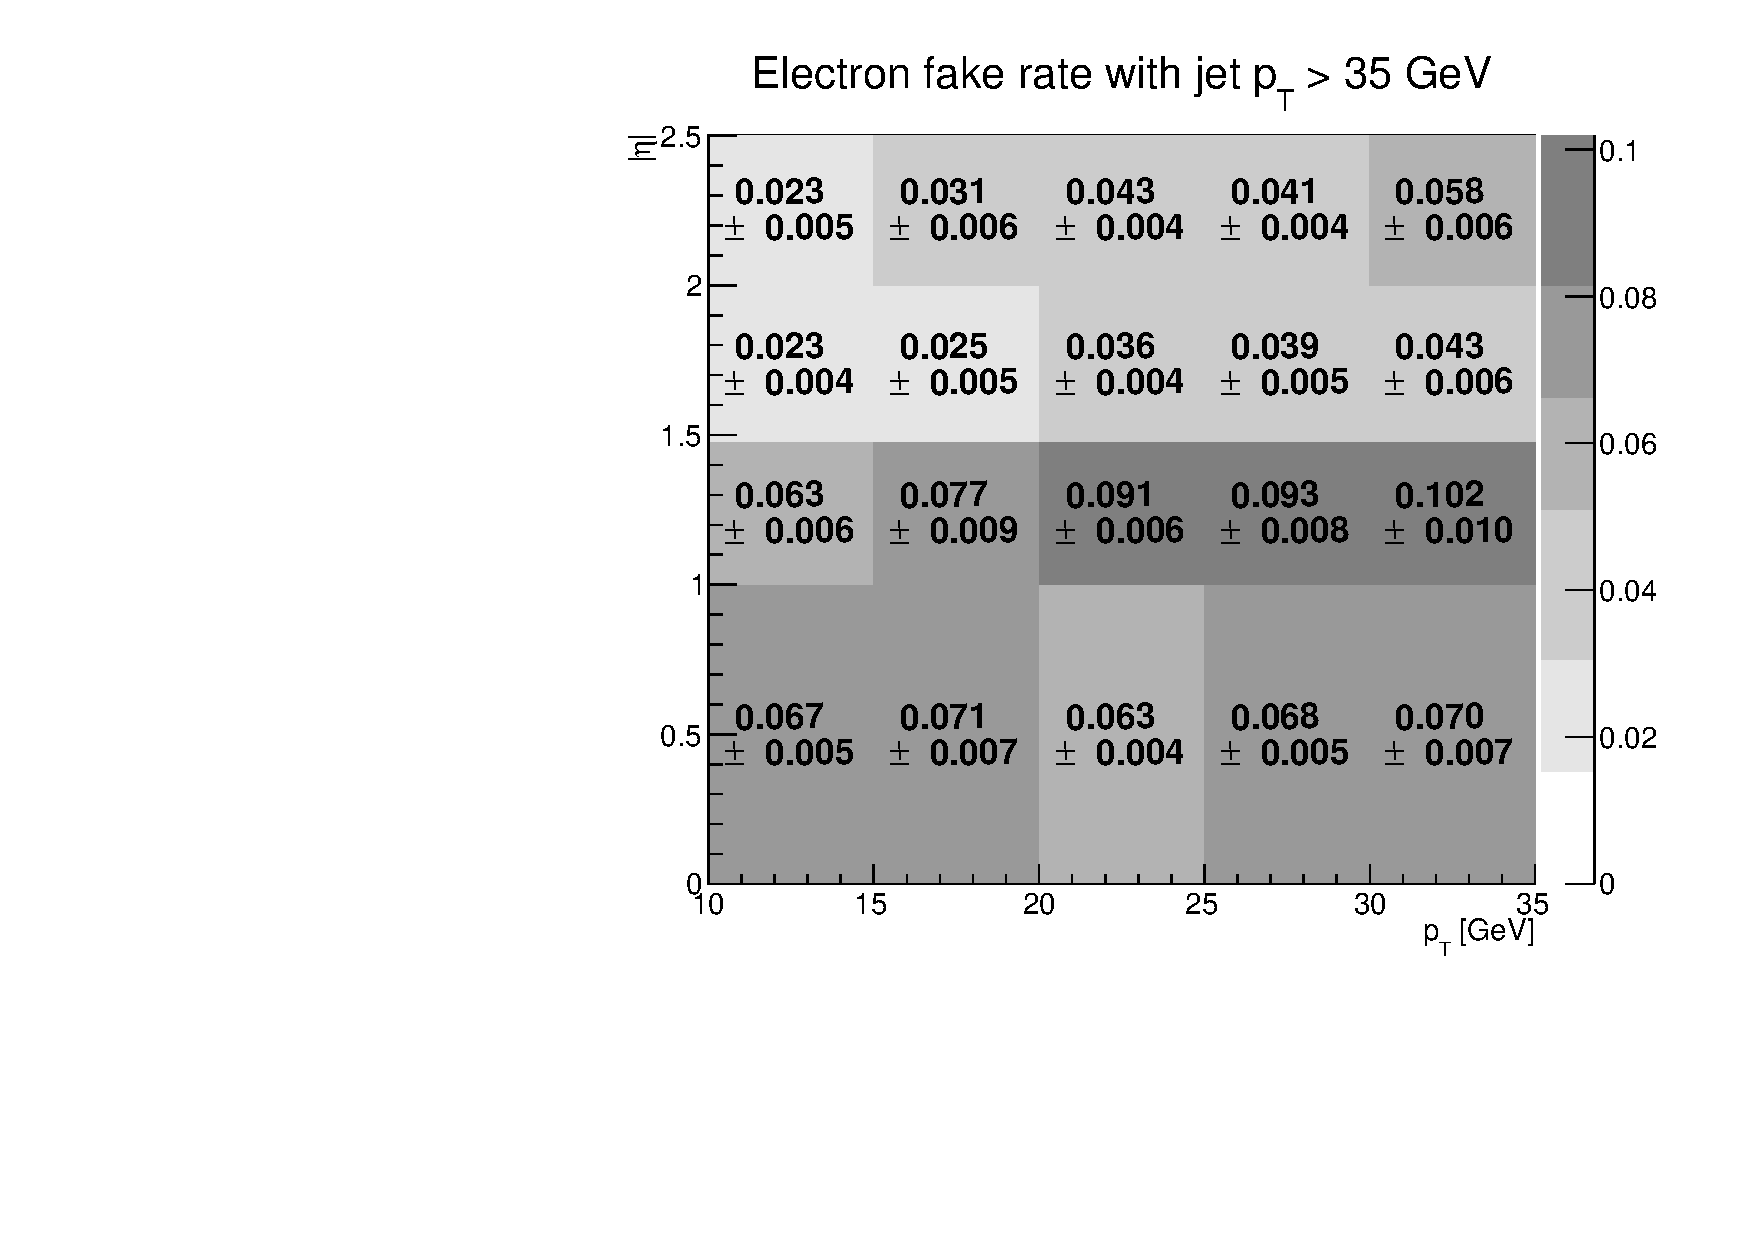
\includegraphics[width=0.75\textwidth]{figures/2DFR_Electron_jet35.pdf}
\end{tabular} 
\caption{Top shows muon fake rate as a function of FO \pt\ and \Eta, 
measured with the away jet $\pt>30~\GeV$.  
Bottom shows electron fake rate as a function of FO \pt\ and \Eta,
measured with the away jet $\pt>35~\GeV$.
The errors are only statistical.}
\label{fig:2DFR} 
\end{figure} 


\subsubsection{Application of fake rate}

The measured FR as a function of \pt\ and \Eta\ of the FO is used to predict the 
contribution of \Wjets\ in the signal region. In data we first select events 
in which one lepton passes the full lepton selection while the other lepton 
passes the FO selection but not the full selection(Tight+Loose sample). 
The contribution from other 
background processes are subtracted in order to get a pure \Wjets\ sample. 
\begin{figure}[htp] 
\centering 
\begin{tabular}{c} 
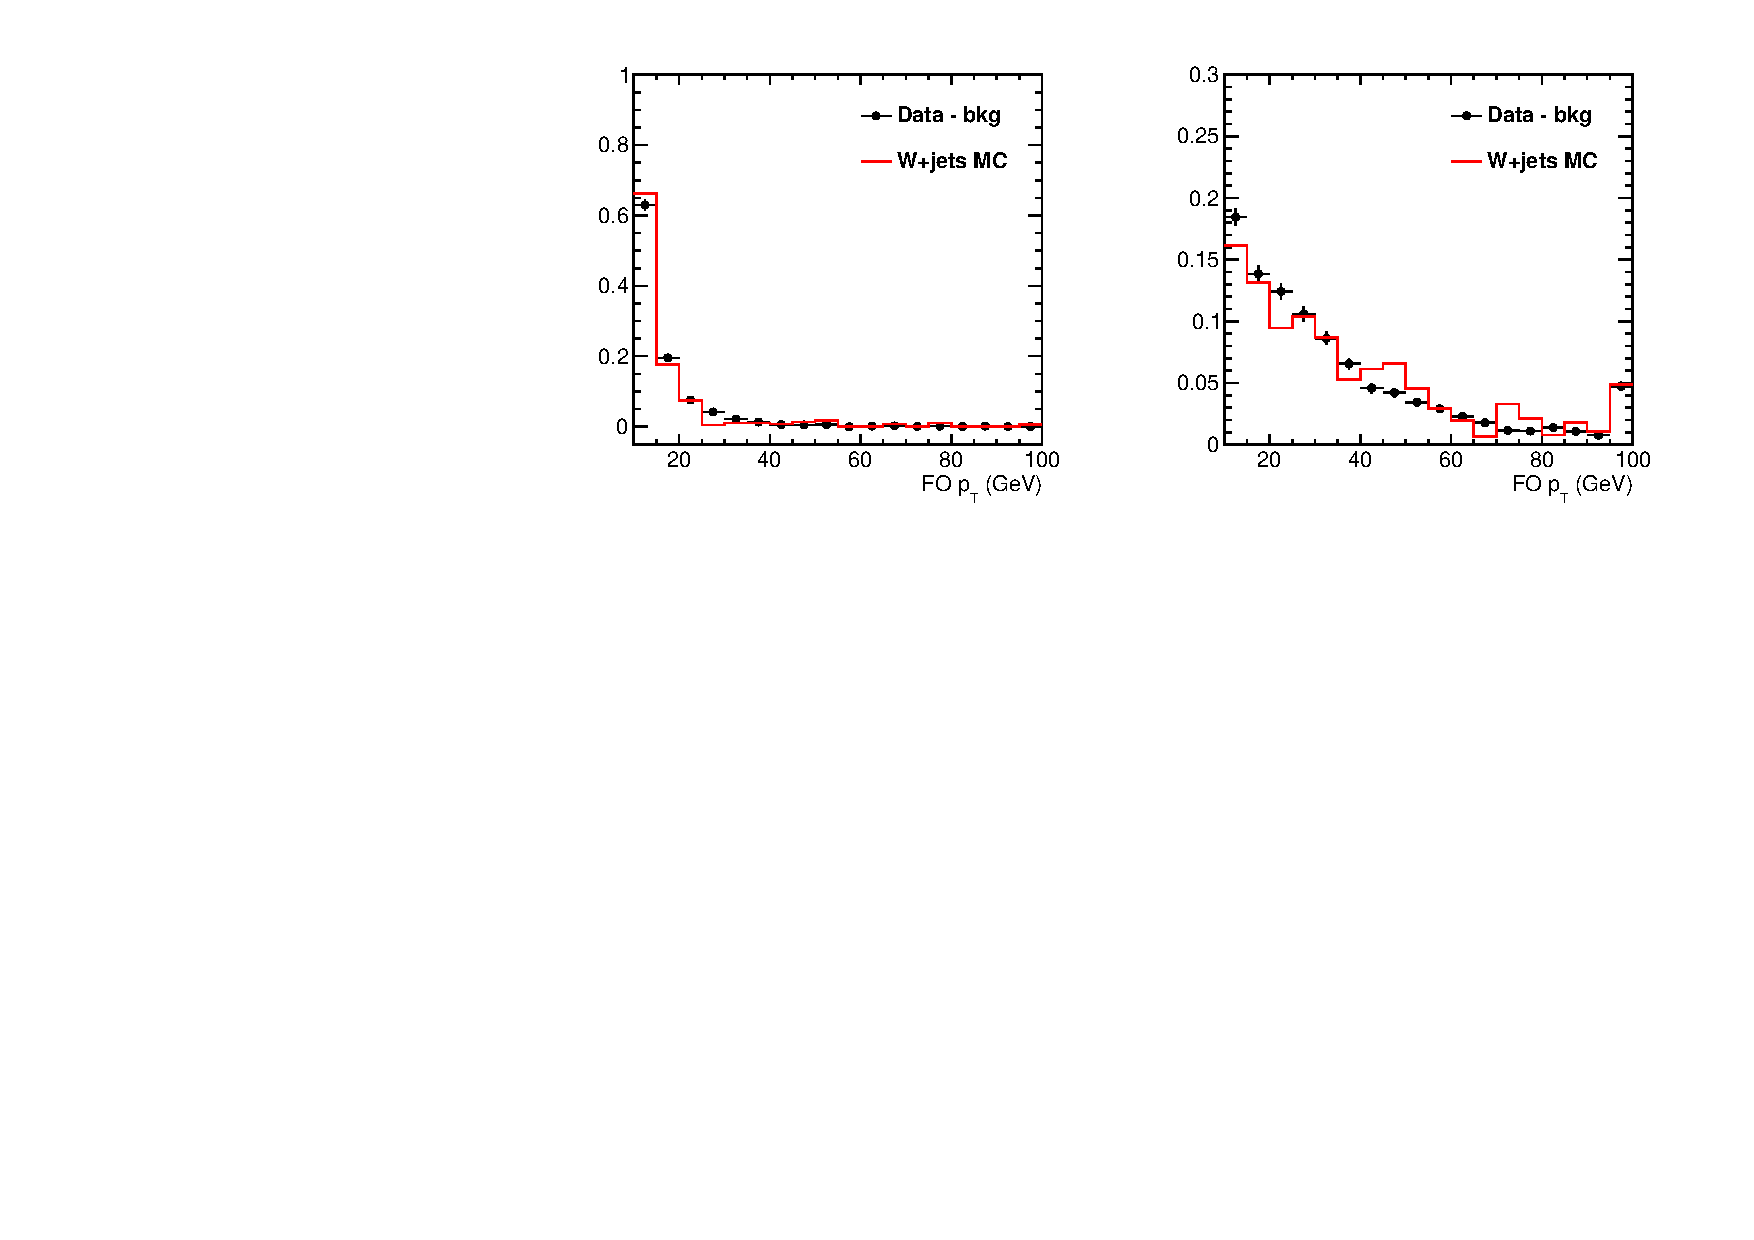
\includegraphics[width=1.00\textwidth]{figures/FOpT_0j_of.pdf} 
\end{tabular} 
\caption{The \pt\ of muon FO (left)and electron FO(right). 
Plots are normalized to the unit area. 
On each plot, the shape of data after subtracting other backgrounds,
and that of \Wjets\ MC are compared. 
They have consistent shapes giving confidence that the selected data sample 
is dominated by \Wjets\ process. } 
\label{fig:FOpT} 
\end{figure} 
Figure~\ref{fig:FOpT} shows the \pt\ distribution of the muon and electron FO
on left and right, respectively. The plots are normalized to the unit area.
The data with other backgrounds subtracted and the \Wjets\ simulation show good
agreement in shape giving confidence that the selected data sample
is dominated by \Wjets\ process. Now we use the measured FR as a weight to the 
Tight+Loose sample in the following way.   
\begin{eqnarray} 
N_{\Wjets}^{\textrm{prediction}} 
= \sum_i^{N_{\textrm{Tight+Loose}}} \frac{\textrm{FR}({\pt}_i, \eta_i)}{1 - \textrm{FR}({\pt}_i, \eta_i)}    
\end{eqnarray} 
where $N_{\Wjets}^{\textrm{prediction}}$ is the prediction of \Wjets\ background 
in the signal region, $N_{\textrm{Tight+Loose}}$ is the number of Tight+Loose events
and ${\pt}_i$ and $\eta_i$ are the \pt\ and \Eta\ of the Loose lepton in the $i^{th}$ 
Tight+Loose event.

\subsubsection{Systematics}
%
\begin{figure}[htp] 
\centering 
\begin{tabular}{c} 
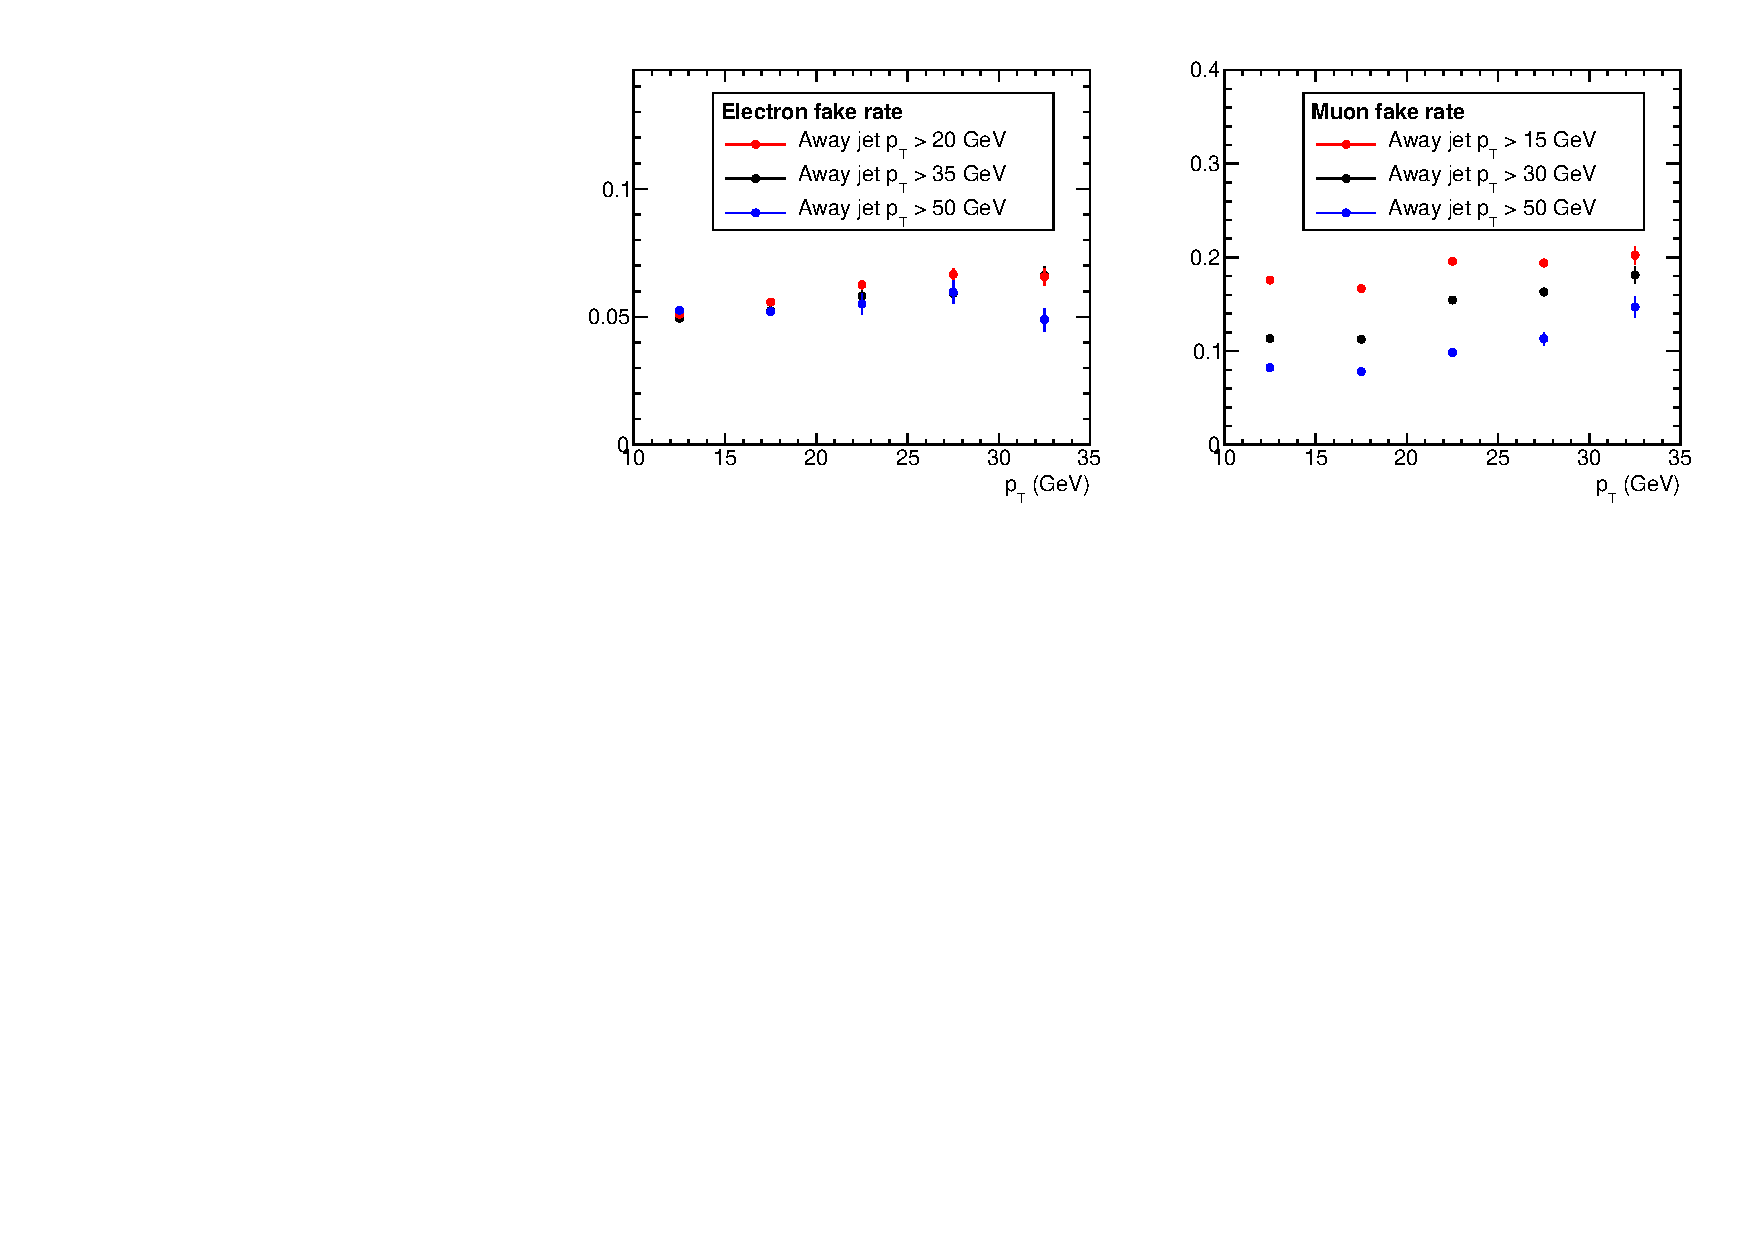
\includegraphics[width=1.0\textwidth]{figures/FR_jetpt_variation.pdf}
\end{tabular} 
\caption{Left plot is the electron fake rates projected on \pt\ for 
different away jet \pt\ thresholds, 20, 35(default) 50~\GeV. 
Right plot is the muon fake rates projected on \pt\ for
different away jet \pt\ thresholds, 15, 30(default) and 50~\GeV.} 
\label{fig:FR_jetpt_variation} 
\end{figure} 
As mentioned before, the away jet \pt\ is a handle for the QCD di-jet events 
to give relevant kinematic range for FO in \Wjets.  
But, it has a limited control of the kinematics of the parton
from which the FO originates. 
We, therefore, assign a systematic uncertainty 
to account for our limitation of controlling the progenitor \pt\ 
by varying the away jet \pt\ threshold
to cover the relevant kinematic range of the \Wjets\ sample.
Figure~\ref{fig:FR_jetpt_variation} shows the dependence of FR on the 
away jet \pt\ thresholds. Left plots shows the dependence of electron 
FR, and the right plot shows the dependence of muon FR. 
The alternative away jet \pt\ thresholds are 20 and 50~\GeV\ for electrons 
and 15 and 50~\GeV\ for muons. The prediction using the alternative \pt\ thresholds
differ by 30 \% compared to the nominal results when electrons and muons are combined, 
and this difference is taken as systematic uncertainty. 
The dependence on the jet \pt\ is larger for muons than electrons. 
This is because of difference in the FO definition. The electron FR is a
dominated by ID requirement which has small dependence on the away jet \pt, 
while the muon FR is dominated by ISO requirement which has strong dependence 
on the away jet \pt.
% WW level 0-jet 
% Ele : 380 ==> 395 : 5 % up
% Mu  : 415 ==> 638 : 50 % up
In addition, the composition of the sample can be different in the QCD di-jet sample 
and the \Wjets\ sample. So, we do a closure test in simulation 
assuming that the parton composition is well-modelled by simulation. 
The result shows that the difference between 
the prediction and the observation is $\sim$ 20 \% for both electrons and muons.
The two systematic uncertainties are combined in quadrature, resulting 
36 \% total systematic uncertainty for both electrons and muons. 
%%%%%%%%%%%%%%%%%%%%%%%%%%
\section{ \topbkg }

The backgrounds induced by top quarks come from \topbkg\ processes where 
the W boson decayed from a top quark decays leptonically. These processes 
result in two isolated leptons with considerable \met, which is 
the signature of signal events, and b-tagged jets which
can be used to suppress this background. However, in case the b-jet 
goes out of the tracker coverage or it is not tagged as a b-jet, 
these events can survive the signal selection. To estimate its 
contribution, We use a data-driven method applied to 0-jet and 1-jet separately.

The top background is estimated after the WW selection and a common 
data/simulation scale factor for \topbkg\ is calculated in 0-jet and 1-jet 
categories. Then, the simulation is normalized by the measured scale factor. 
The basic idea of the top estimation is to re-weight the top-tagged control region 
using the top-tagging efficiency obtained from an independent sample. This 
can be expressed as the following equation, 
\begin{eqnarray} 
N_\textrm{top-veto} 
= 
N_{\textrm{top-tagged}} \times
\frac{1 - \epsilon_{top-tagging}}{\epsilon_{top-tagging}}   
\end{eqnarray} 
where $N_\textrm{top-veto}$ is the prediction for the top-vetoed events 
in the signal region, $N_{\textrm{top-tagged}}$ is the number of 
the top-tagged events which can be obtained by inverting the top-veto requirement, 
and $\epsilon_{top-tagging}$ is the top-tagging efficiency 
measured in an independent data sample. The top-tagging efficiency 
is measured in a different way in the 0-jet and the 1-jet categories.
Table~\ref{tab:topbkgest} shows the definition of the control region 
and the tagging efficiency in the 0-jet and the 1-jet categories.

\begin{table}[!h]
\begin{center}
\footnotesize
\label{tab:topbkgest}
\vspace{0.5cm} 
\caption{Summary of selection and control region definitions used 
in top estimation in the different jet bins.}
\vspace{0.5cm} 
\begin{tabular} {|c|c|c|c|c|}
\hline
jet bin & signal region & control region & \multicolumn{2}{c|}{$\epsilon_{tag}$}  \\  
        \cline{4-2} \cline{5-2} 
        & (top veto)    & (top tag)      & denominator & numerator \\ 
\hline
0       & no soft muon,      & either a soft muon  & 1-jet bin, leading & denom. + \\
        & no low \pt\ b-jets & or a low \pt\ b-jet & jet is btagged     & top tag  \\
\hline
1       & no soft muon,           & leading jet  & 2-jet bin, sub-leading & denom. + \\
        & no low/high \pt\ b-jets & is b-tagged  & jet is btagged         & top tag  \\
\hline
\end{tabular}
\end{center}
\end{table}

\subsubsection{0-jet category method}

We start with measuring the ``per-leg" tagging efficiency, 
which is the probability for a b quark to be tagged.
In the \ttbar\ events, there are two b quarks in the final states, 
so we can explore the second b quark after requiring that the first b quark be tagged. 
A caveat is that the \tw\ contribution should be subtracted because
those events have only one b quark in the final state, and the second 
jet is from FSR or ISR regardless of jet flavors. 
Some of the FSR or ISR jets can be b-tagged as well, and this 
makes \tw\ indistinguishable from \ttbar. Therefore, this should 
be accounted for when calculating the ``per-event" top-tagging efficiency. 

For the denominator the ``per-leg" efficiency is defined 
by requiring exactly one b-tagged jet with $\pt>30~\GeV$. 
This requirement is to select a sample dominated by \topbkg.  
Of the selected events, a subset of events containing at least one b-tagged jet
with $10<\pt<30~\GeV$ or one soft-muon becomes the numerator. 
The ratio of the yields in the numerator to the denominator after subtracting contributions 
from other backgrounds as well as \tw\ is the ``per-leg" top-tagging efficiency, 
$\epsilon_{per-leg}^{data}$. 

The ``per-event" top-tagging efficiency is then calculated by the following equation, 
\begin{eqnarray} 
\label{eq:TopTagEff0jet}
\epsilon_{\textrm{top-tag, per-event}}^{data} 
= 
\begin{array}{ccc} \multicolumn{2}{c}{\displaystyle 
\left(1-\left(1-\epsilon_{per-leg}^{data}\right)^2\right) 
\left(f_{t\bar{t}}^{MC} + x\left(1-f_{t\bar{t}}^{MC}\right) \right)
} & \\ & \multicolumn{2}{c}{\hspace{5cm} \displaystyle
+ \left(1-f_{t\bar{t}}^{MC}\right)\left(1-x\right)\epsilon_{per-leg}^{data}
} \end{array}   
\end{eqnarray} 
where the first term corresponds to the tagging efficiency for the events with 
two taggable legs, and the second term corresponds to the tagging efficiency for 
the events with one taggable jet. 
The $\epsilon_{\textrm{top-tag, per-event}}^{data}$ is the per-event top-tagging efficiency. 
The $f_{t\bar{t}}^{MC}$ is the fraction of \ttbar\ events with respect to the 
\ttbar+\tw\ events measured using MC at WW level requiring no jets. 
The $x$ is the fraction of events that contain two taggable legs in \tw\ events. 
It corresponds to the $\epsilon_{per-leg}$ measured in \tw\ MC.  

Finally, the control region in data is defined by inverting the top-veto requirement, 
\textit{i.e.}, requiring soft-muon or b-tagged jets with $10<\pt<30~\GeV$.
The contributions from other backgrounds are subtracted so that the 
measured top-tagging efficiency is applied to only \topbkg\ events. 
The left plot in Figure~\ref{fig:TCHE_topCR} shows the level of agreement between 
data and MC in the top control region for 0-jet category.  
They show good agreement, and we conclude that the data subtracted by other backgrounds 
will give \topbkg\ events with high purity. 
The prediction of \topbkg\ events in the signal region is calculated by 
\begin{eqnarray} 
\label{eq:topExtrapolation0jet}
N^{top}_{\textrm{WW region}}
%&=&  
%N_{top-tag}^{\textrm{top CR, \topbkg}} \times
%\frac{1-\epsilon_{\textrm{top-tag, per-event}}^{\textrm{data}}}
%     {\epsilon_{\textrm{top-tag, per-event}}^{\textrm{data}}} \\ 
&=&   
(N_{top-tag}^{\textrm{data}}-N_{top-tag}^{\textrm{other bkg}}) \times
\frac{1-\epsilon_{\textrm{top-tag, per-event}}^{\textrm{data}}}
     {\epsilon_{\textrm{top-tag, per-event}}^{\textrm{data}}}.  
\end{eqnarray} 
where $N_{top-tag}^{\textrm{data}}$ is the data count in the top CR 
and $N_{top-tag}^{\textrm{other bkg}}$ is the contribution from other 
background process in the top CR.

The systematic uncertainty to the top estimation in the 0-jet category 
is dominated by the uncertainty to the parameter $x$. The uncertainties
of \ttbar\ and \tw\ cross sections are about 7~\% and 15~\%~\cite{Kidonakis:2012rm}, 
and the resulting uncertainty of $x$ is 17~\%. 

\subsubsection{1-jet category method}

The method for measuring top-tagging efficiency for 1-jet category is 
based on the fact that the b-tagging efficiency of the most energetic jet 
in 1-jet and 2-jet categories is approximately same. The efficiencies 
measured in \ttbar\ MC after WW selection is 66 \% and 67 \% in 1-jet 
and 2-jet categories, respectively. Therefore, we measure the b-tagging 
efficiency($\epsilon_{\textrm{top-tag, per-event}}^{\textrm{data}}$) 
of the most energetic jet in events containing 2-jets,
and apply this to the control region in the 1-jet category.  
The definition of control region is different from an inversion of 
the top-veto requirement in this case because the b-tagging efficiency 
is correlated with existence of soft-muons in the jet. 
So, the control region is defined without soft-muon requirement, 
and this definition is consistently applied for the top-tagged region, 
top-vetoed region and the top-tagging efficiency measurement.
The right plot in Figure~\ref{fig:TCHE_topCR} shows the level of agreement between 
data and MC in the top control region in the 1-jet category.  
They show a good agreement, and we conclude that the data subtracted by other backgrounds 
gives \topbkg\ events with high purity. 

Then, the top contribution in WW region is calculated using the measured
top-tagging efficiency($\epsilon_{\textrm{top-tag, per-event}}^{\textrm{data}}$) 
and the number of events in the top CR($N_{top-tag}^{\textrm{data}}
-N_{top-tag}^{\textrm{other bkg}}$) as shown in the equation~\ref{eq:topExtrapolation0jet}.

\begin{figure}[htp] 
\centering 
\begin{tabular}{c} 
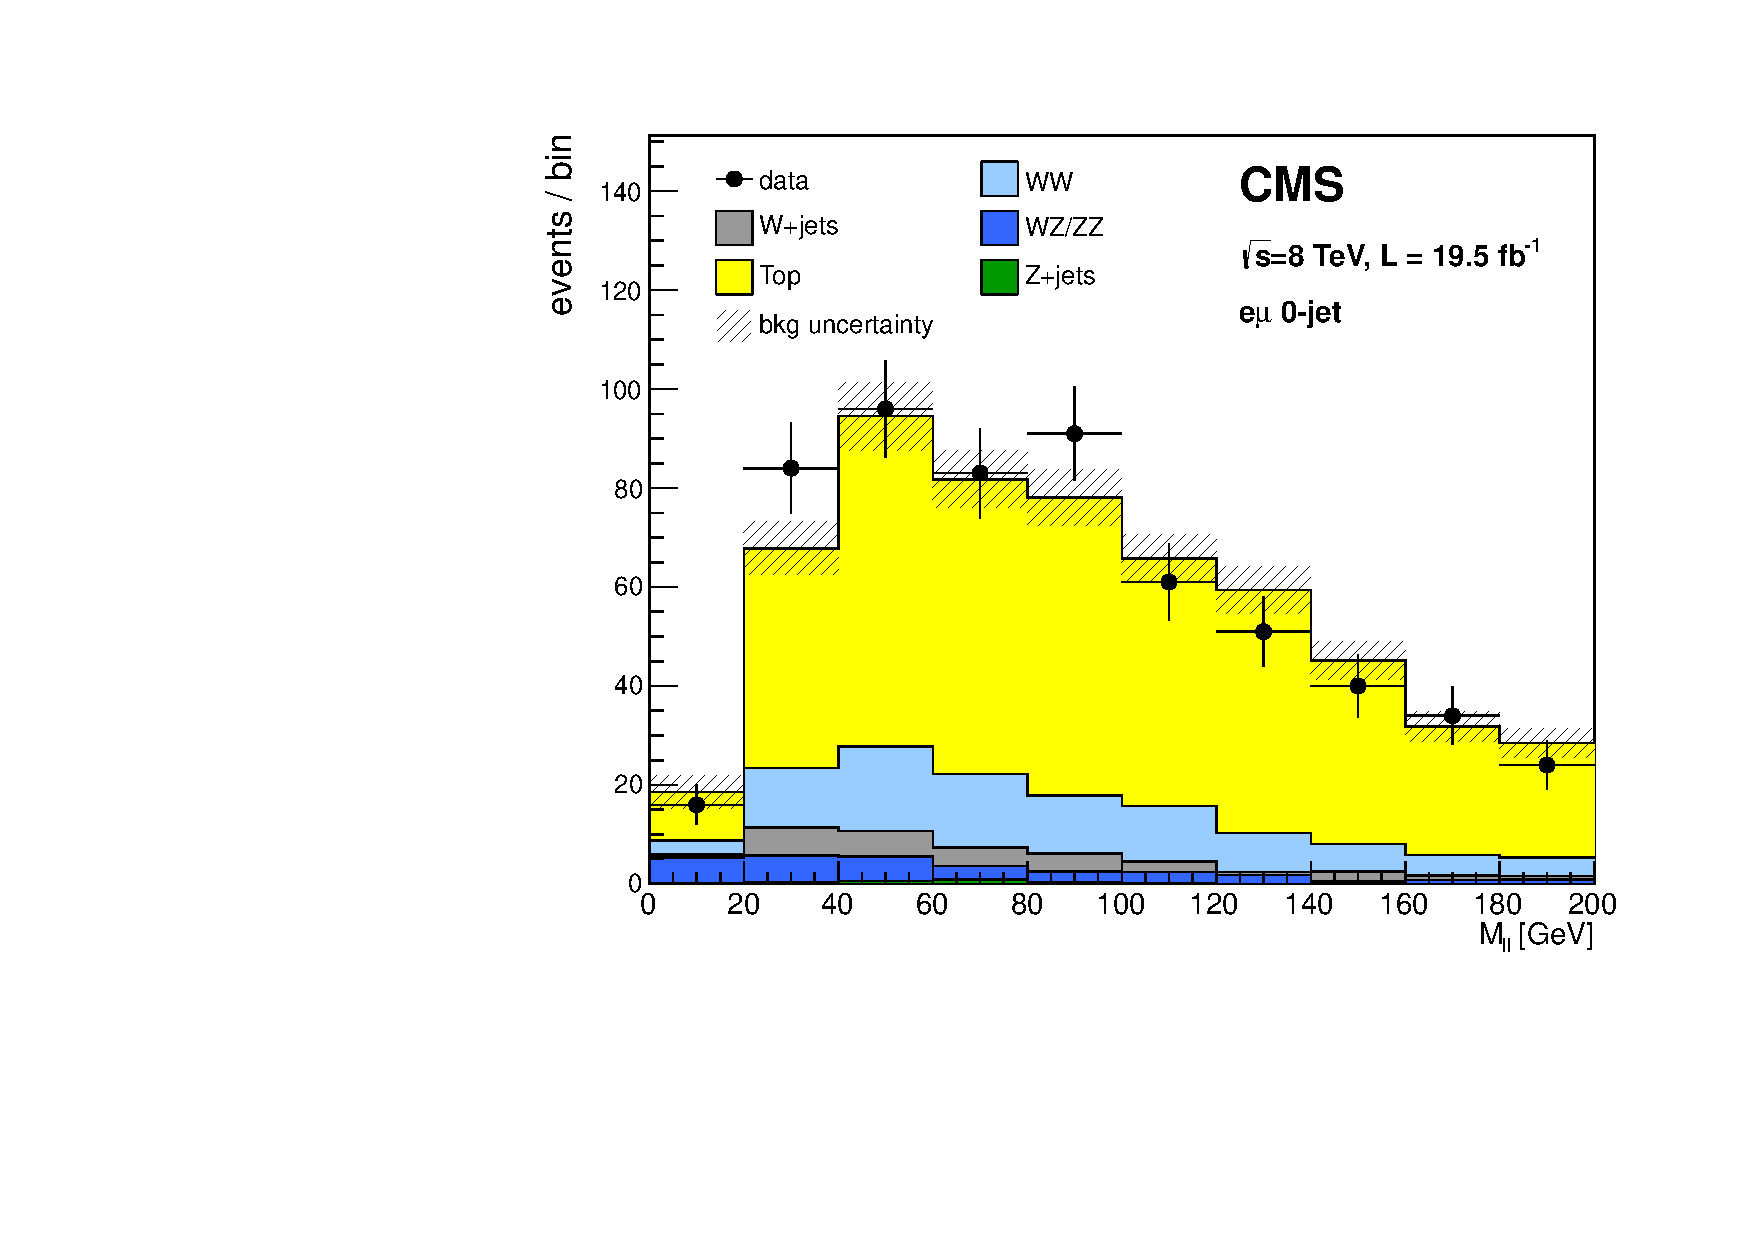
\includegraphics[width=0.5\textwidth]{figures/topcontrol_mll_of_0j.pdf}
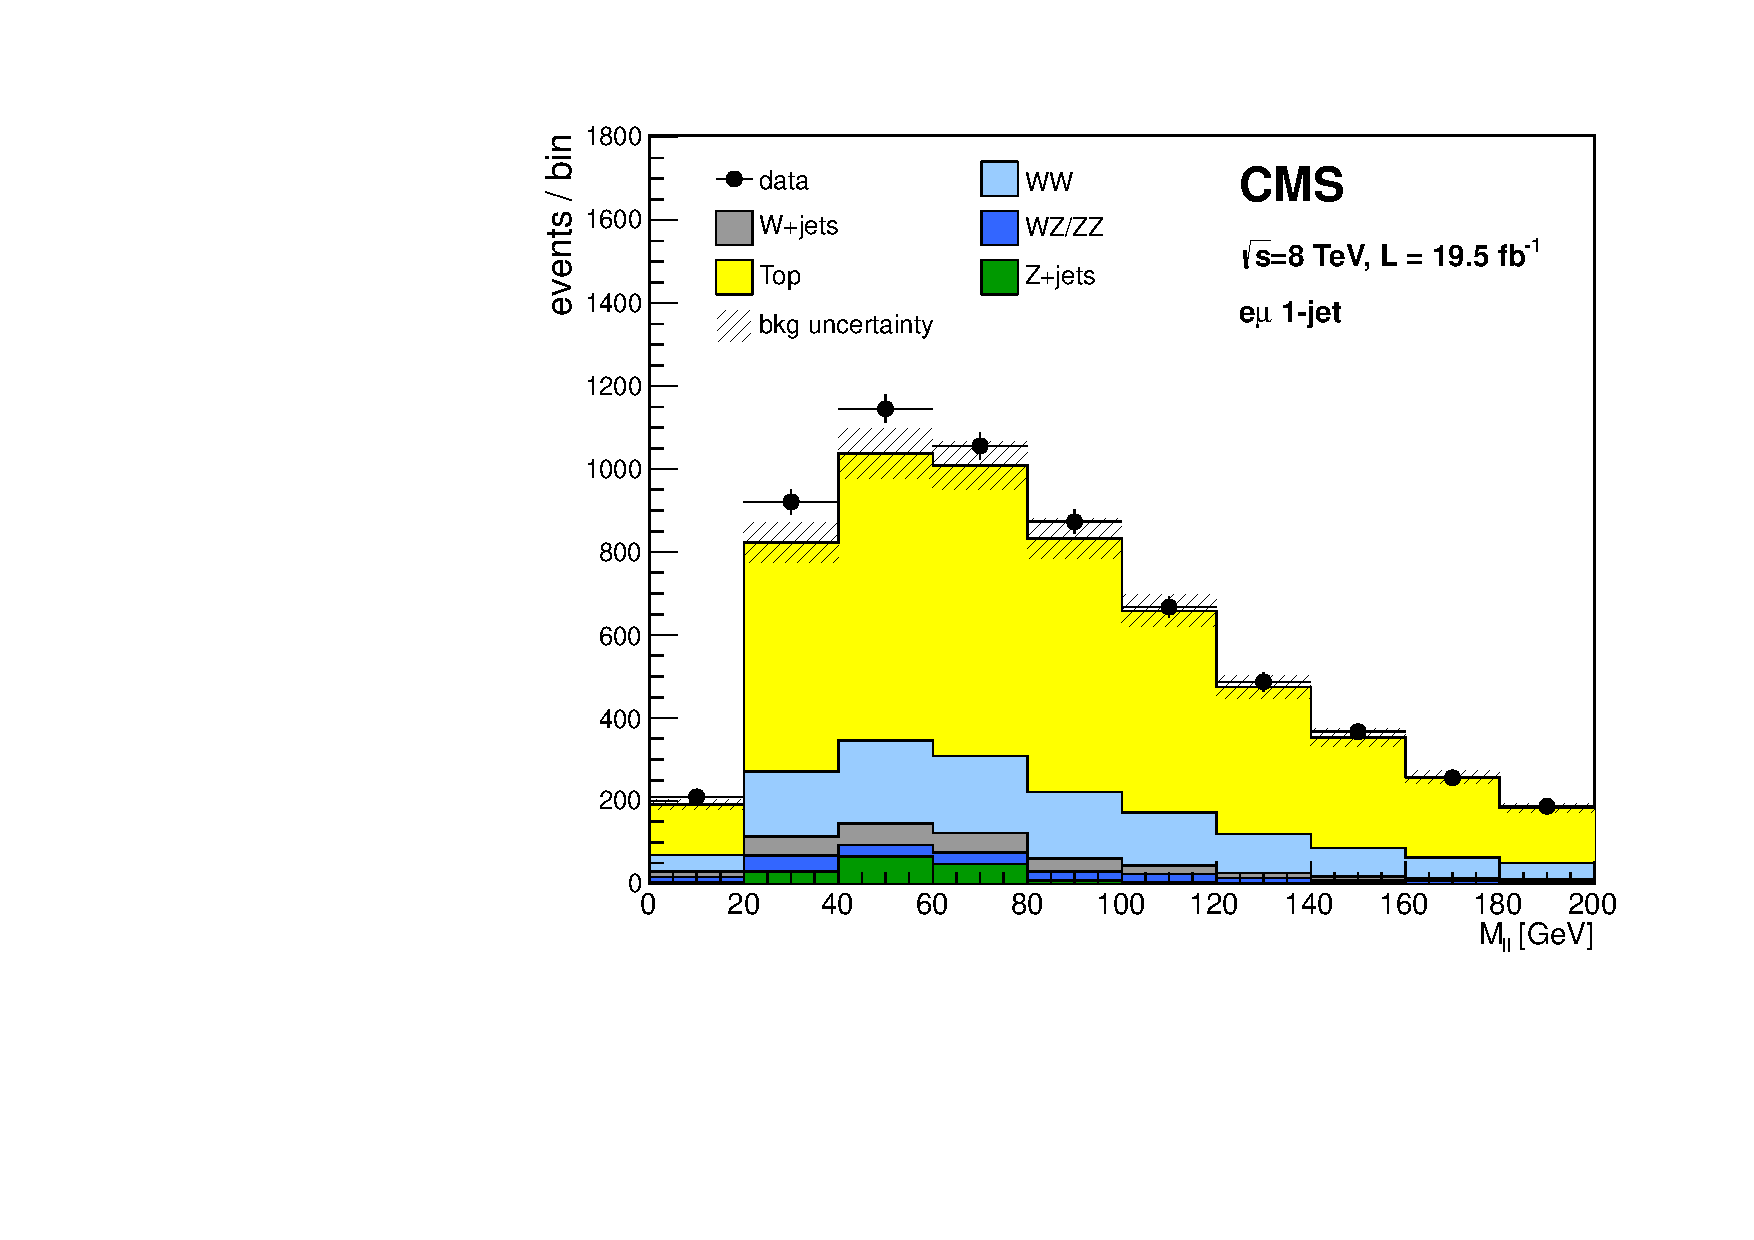
\includegraphics[width=0.5\textwidth]{figures/topcontrol_mll_of_1j.pdf} 
\\
\includegraphics[width=0.5\textwidth]{figures/topcontrol_mt_of_0j.pdf}
\includegraphics[width=0.5\textwidth]{figures/topcontrol_mt_of_1j.pdf} 
\\
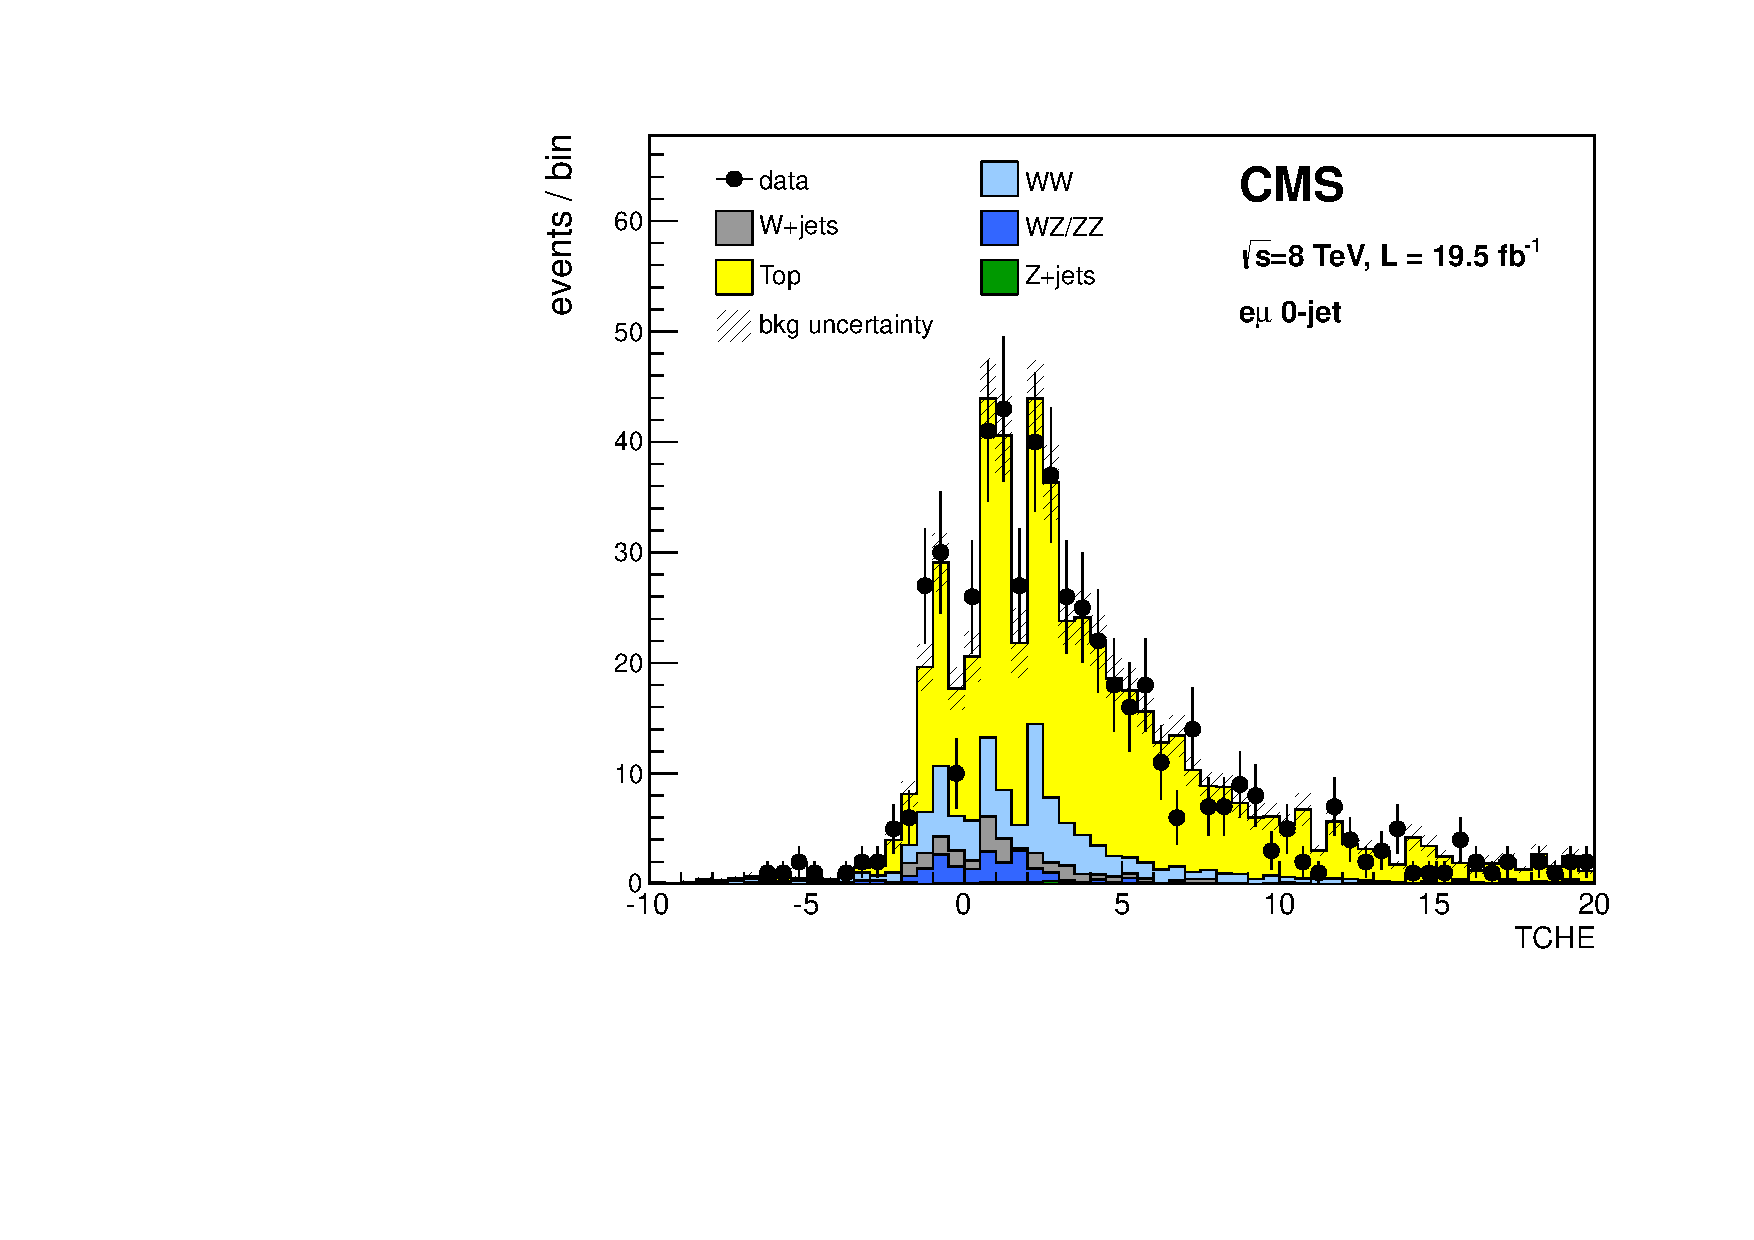
\includegraphics[width=0.5\textwidth]{figures/topcontrol_tche_of_0j.pdf}
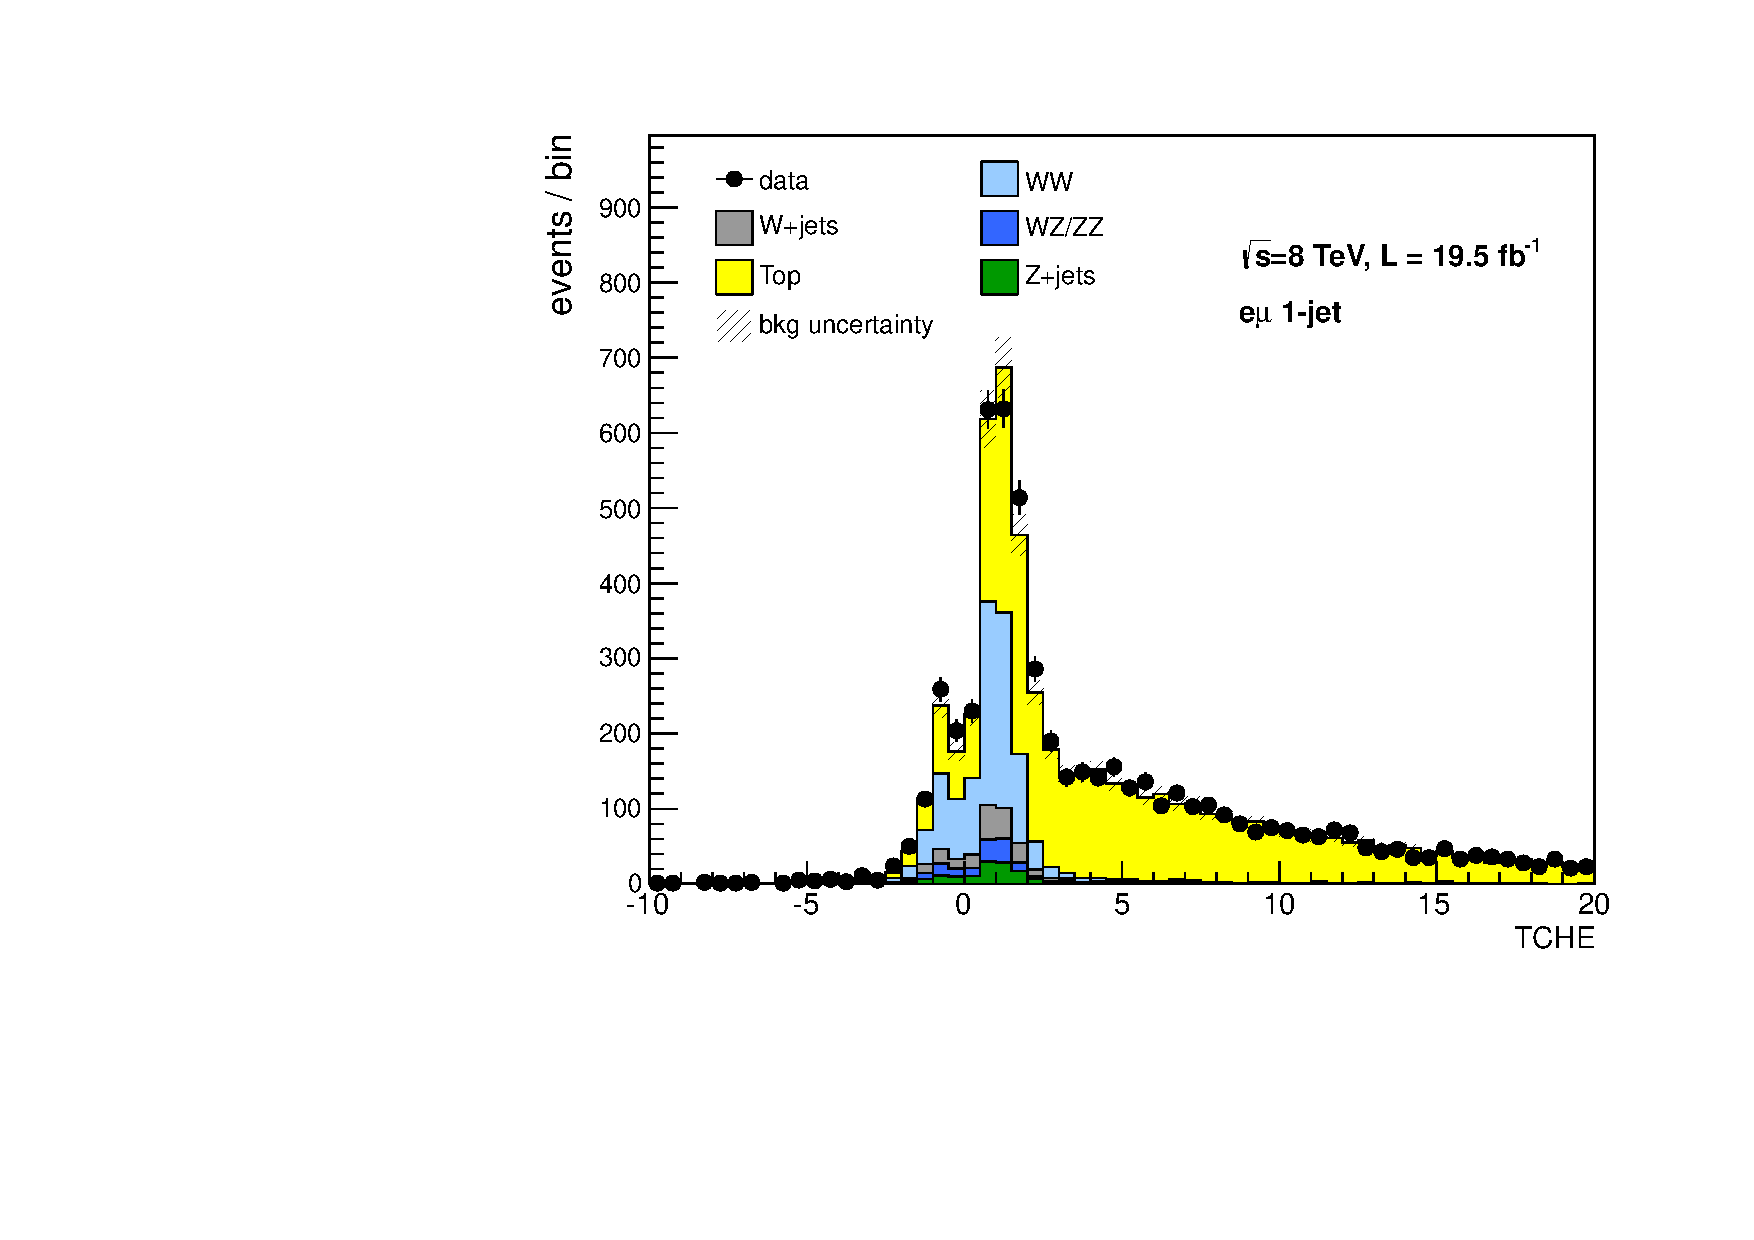
\includegraphics[width=0.5\textwidth]{figures/topcontrol_tche_of_1j.pdf} 
\end{tabular} 
\caption{Distribution of b-tagging discriminator for most energetic jet($\pt>10~\GeV$) 
in the event in the 0-jet(left) and 1-jet(right) top control regions
where top-tagging efficiency is measured. The agreement between data and MC is good, 
and it shows good control of \topbkg\ in the data.} 
\label{fig:TCHE_topCR} 
\end{figure} 

The systematic uncertainty to the top estimation in the 1-jet category 
is dominated by data statistics in the control region which accounts for 
about 2~\%.     

\subsubsection{Result}

Table~\ref{tab:ttbar_est} shows the result of the data-driven estimation for \topbkg. 
The data/simulation scale factors are consistent to unity in both 0-jet and 1-jet categories. 
The uncertainty is large in the 0-jet category due to the large cross section uncertainty 
of the \tw\ process. The calculated scale factors are applied to the MC counts 
in the signal region.

\begin{table}[ht!]
\begin{center}
\label{tab:ttbar_est}
\vspace{0.5cm} 
\caption{Monte Carlo to data scale factor for the top background contribution 
for $\intlumiEightTeV$.} 
\vspace{0.5cm} 
\begin{tabular}{c c c}
\hline
                             Sample     & 0-jet                   & 1-jet               \\
\hline
Estimated \topbkg events in simulation  & 720.5 $\pm$   4.3 & 2151.3 $\pm$  13.9        \\
Tagging efficiency     (\%)             & 49.3 $\pm$  4.3   & 64.8 $\pm$  0.5           \\ 
Data events in control region           & 1034              & 4847                      \\ 
Background events in control region     & 292.6 $\pm$  43.9 & 255.5 $\pm$  51.1         \\ 
\topbkg estimation in data              & 761.4 $\pm$ 146.5 & 2307.9 $\pm$  59.4        \\
Data/simulation scale factor            & 1.06 $\pm$  0.20  & 1.07 $\pm$  0.03          \\
\hline
\end{tabular}
\end{center}
\end{table}

%%%%%%%%%%%%%%%%%%%%%%%%%%
\section{ \ww }
\begin{figure}[htp] 
\centering 
\begin{tabular}{c} 
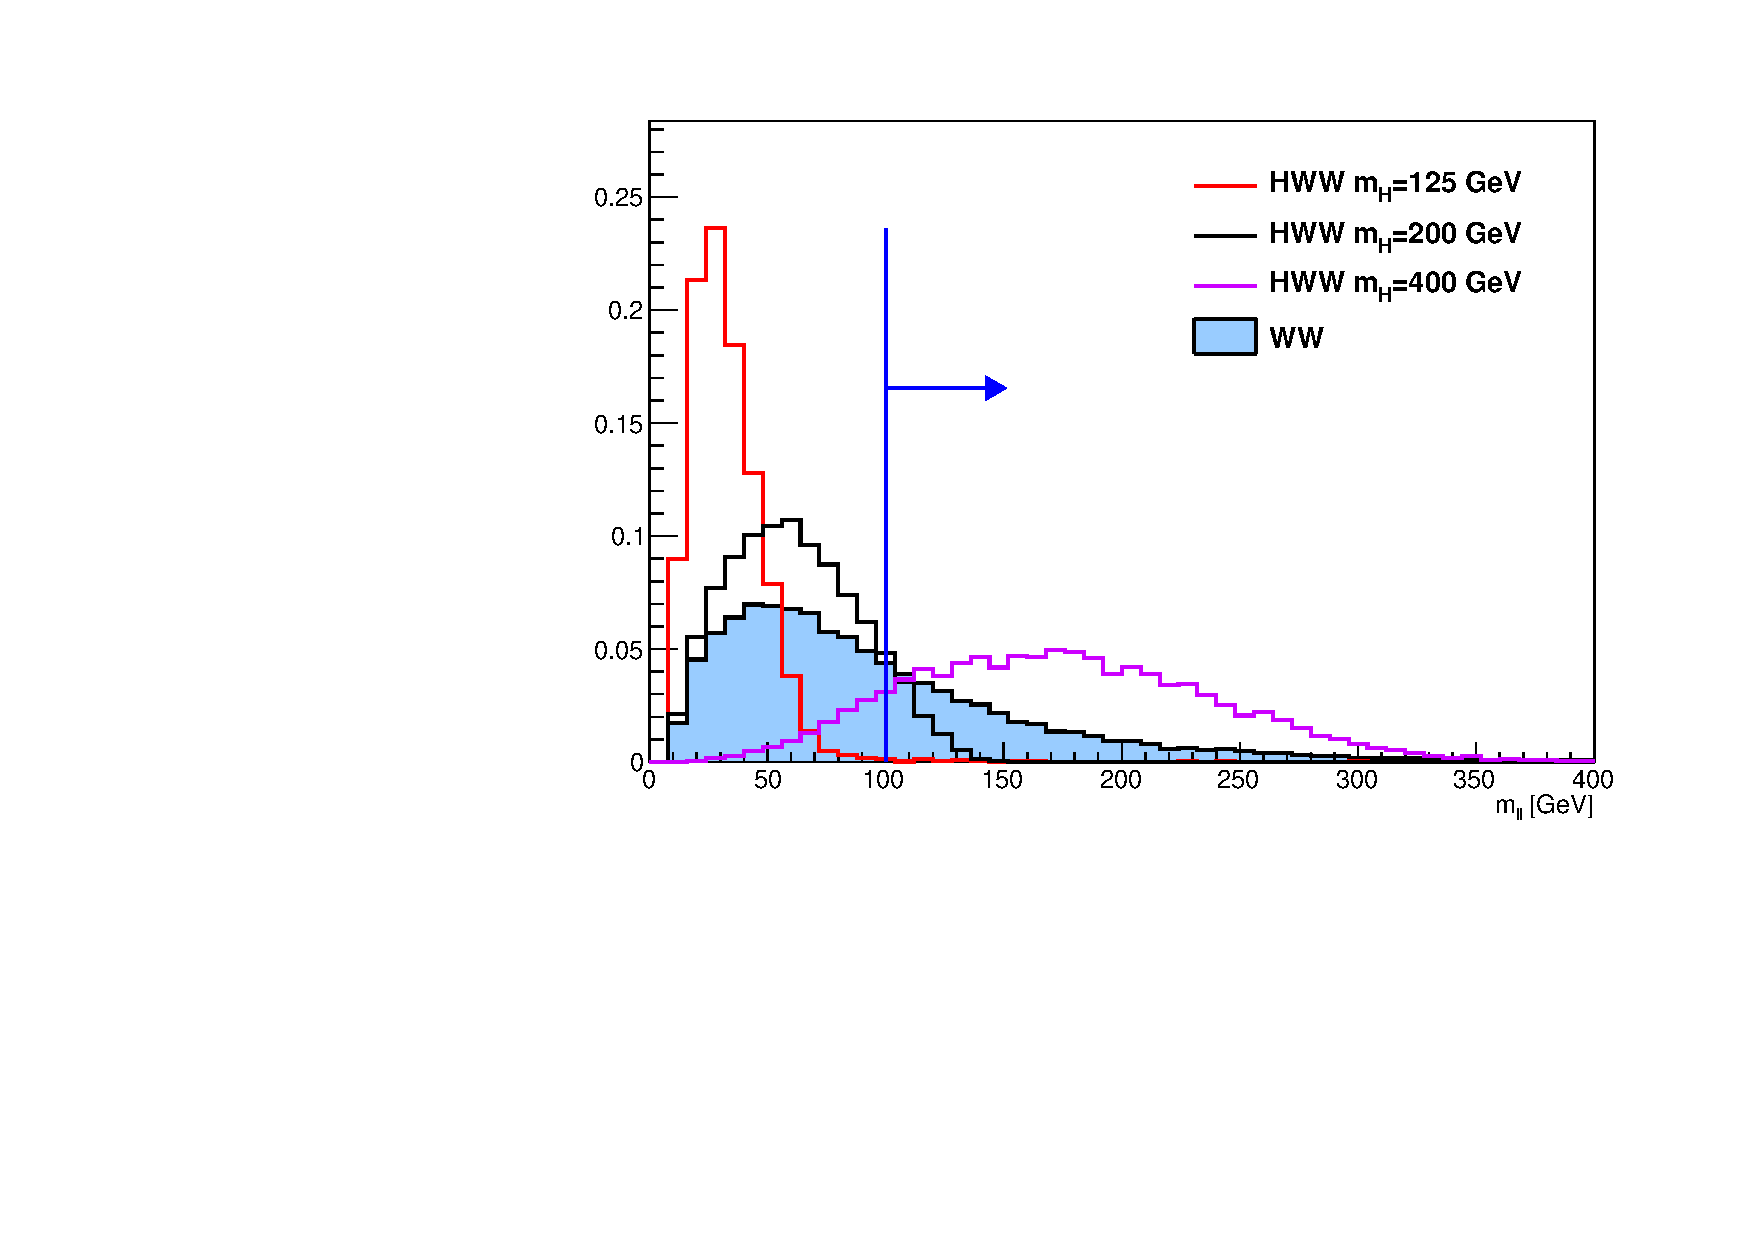
\includegraphics[width=1.0\textwidth]{figures/WW_mll_0j_of.pdf} 
\end{tabular} 
\caption{ \mll\ distributions in 0-jet \DF\ channel for various signal events, 
\mHi=125, 200 and 400~\GeV\ and WW after WW selection. The control region, $\mll>100~\GeV$, 
is marked with a blue line.} 
\label{fig:WW_mll} 
\end{figure}  

The non-resonant \WW\ background is the main background in the most sensitive 
category(0-jet \DF)and estimated for 0-jet and 1-jet categories separately 
using the \mll\ distribution.
Figure~\ref{fig:WW_mll} shows the \mll\ distributions in 0-jet \DF\ 
category for various \mHi\ points, 125, 200 and 400~\GeV, and WW after WW selection. 
For \mHi\ hypotheses below 200~\GeV, 
there is a negligible contribution from signal in the $\mll>100~\GeV$ region. 
Therefore, this region can be used as a WW control region.  
But, \mHi\ hypotheses above 200~\GeV\ give a significant contamination in that region,
and it can not be used as a control region. So, we rely on simulation
to estimate WW contribution in the signal region for the high \mHi\ hypotheses($\mHi>200~\GeV$). 
For the estimation of WW background in the signal region 
for low \mHi\ hypotheses($\mHi\le200~\GeV$), 
we have different approaches for the shape-based and the cut-based methods. 

For the shape-based method, we measure the data/simulation scale factor 
applying the template selection. 
In this method we expect that fit can constrain the WW component using 
the WW sideband region, \textit{i.e.,} high \mT\ and/or high \mll\ region. Therefore,   
the measured scale factor is used to set the initial point for the fit to start. 
The \textit{pdf} for the WW normalization in the fit model is a flat function, 
so its value and the uncertainty are entirely determined by fit. 

For the cut-based method, we define a control region in the \mll\ space where 
negligible signal events are expected, and extrapolate the control region yield 
to the signal region using the ratio of signal region to control region calculated 
in simulation($R_{\textrm{SR/CR}}$). 
At each \mHi\ hypothesis, the control region is defined with the \pt\ requirements 
on the leading and the trailing leptons on top of $\mll>100~\GeV$. 

The following equation summarizes how the estimation is done, 
\begin{eqnarray} 
N_{\textrm{WW}}^{\textrm{SR}} 
&=&  
\left( N_{\textrm{CR}}^{\textrm{data}}  
     - N_{\textrm{CR}}^{\textrm{other bkg}}\right) \times R_\textrm{SR/CR}^{\textrm{MC}}.  
\end{eqnarray} 
We first measure the ratio($R_\textrm{SR/CR}^{\textrm{MC}}$) of events in the signal region 
to the control region using simulation.  
Then, we obtain the yield($N_{\textrm{CR}}^{\textrm{data}}$) in the 
control region($\mll>100~\GeV$) in data, and subtract the contribution from other 
backgrounds($N_{\textrm{CR}}^{\textrm{other bkg}}$) such as \topbkg, \Wjets\ and \dyll.  
The data-driven estimation described in the previous sections are used for 
these backgrounds. Other small backgrounds are taken from simulation. 
We multiply the extrapolation factor to the data yield in the CR 
to get the prediction of WW in the signal region($N_{\textrm{WW}}^{\textrm{SR}}$).
The same data/simulation scale factor is used for \qqww\ and \ggww\ to scale 
the prediction by simulation. 

The uncertainty on the scale factor comes from the statistics in data control region
and the systematic uncertainty of the other background in the control region. These two sources
contribute almost equally to the final uncertainty. Table~\ref{tab:WWest} shows the result 
of the data-driven estimation of WW background. 
\begin{table}[ht!]
\begin{center}
\label{tab:WWest}
\vspace{0.5cm} 
\caption{The result WW background estimation for cut-based and shape-based analyses.}
\vspace{0.5cm} 
\begin{tabular}{c | c | c } 
\hline
\multirow{2}{*}{mass [\GeV]} & 0-jet        & 1-jet \\
                             & scale factor & scale factor \\
\hline
\multicolumn{3}{c}{Cut-based} \\
\hline
 115 &  1.10  $\pm$  0.06  &  0.93  $\pm$  0.10 \\
 120 &  1.10  $\pm$  0.06  &  0.93  $\pm$  0.10 \\
 125 &  1.10  $\pm$  0.06  &  0.93  $\pm$  0.10 \\
 130 &  1.10  $\pm$  0.06  &  0.93  $\pm$  0.10 \\
 135 &  1.10  $\pm$  0.06  &  0.93  $\pm$  0.09 \\
 140 &  1.10  $\pm$  0.06  &  0.93  $\pm$  0.09 \\
 150 &  1.08  $\pm$  0.06  &  0.93  $\pm$  0.10 \\
 160 &  1.08  $\pm$  0.06  &  0.93  $\pm$  0.10 \\
 170 &  1.07  $\pm$  0.06  &  0.92  $\pm$  0.10 \\
 180 &  1.07  $\pm$  0.06  &  0.92  $\pm$  0.10 \\
 190 &  1.07  $\pm$  0.06  &  0.92  $\pm$  0.10 \\
 200 &  1.07  $\pm$  0.06  &  0.91  $\pm$  0.10 \\
\hline \hline
\multicolumn{3}{c}{Shape-based} \\
\hline
All masses & 1.19  $\pm$  0.06  &  1.09  $\pm$  0.10 \\
\hline
\end{tabular}
\end{center}
\end{table}


%%%%%%%%%%%%%%%%%%%%%%%%%%
\section{ \wgammastar }


In the \wgammastar\ events, the leptons decayed from $\gamma^*$ tend to have 
a small opening angle and a small invariant mass, and at least one of them 
has average \pt\ of 5~\GeV. If the conversion happens early in the detector, 
\textit{i.e.}, close to the interaction point,  
and most of the momentum of $\gamma^*$ is carried by one lepton, the other 
lepton may not have enough energy to reach ECAL or muon station. 
In this case that soft lepton can not be reconstructed, and the event 
contains two leptons(one from W and the other from $\gamma^*$) from interaction point 
and \met\ from leptonic W decay. 

The \wz\ simulation is supposed to cover the \wgammastar\ as a part of it, 
but the low $m_{\gamma^*}$ region is not covered appropriately due to the generator 
level cut $m_{\gamma^*}>12~\GeV$. The problem is that there is a significant 
contribution from that region of phase space all the way down to the 
production threshold, $m_{\gamma^*}=2m_{e/\mu}$, to the signal region.
So, we have a dedicated MC sample that was generated in LO to cover this region.
Because it was generated in LO, it is important to measure the k-factor 
to obtain a correct normalization. The k-factor also would tell about the 
validation of the sample. For example, if k-factor is 10, this would indicate 
that the sample is not correctly generated.

When measuring the k-factor, we consider separately 
the cases where the $\gamma^*$ decays to a pair of electrons or muons. 
We use only $l^\pm\mu^+\mu^-$ final state 
because of the uncontrollable QCD backgrounds in the $l^\pm e^+ e^-$ final state. 
We first define a control region dominated by the \wgammastar\ events. 
The following requirements are imposed to define the control region :  
\begin{itemize} 
\item The muon pair should have opposite charges. In case of $\mu^\pm\mu^+\mu^-$ final states, 
      the pair with lowest $m_{\mu\mu}$ is considered coming from $\gamma^*$.
\item The muon isolation is redefined such that it does not include muons in the isolation 
      energy calculation in order to reconstruct $\gamma^*$ from a muon pair very close to 
      each other($\Delta R < 0.3$)
\item To suppress \topbkg, the number of jets should be less than 2, and events containing at least 
      one b-tagged jets with $\pt>10~\GeV$ are excluded
\item To suppress QCD background, $\met>25~\GeV$ and $\mT(W)>45~\GeV$ are applied 
\item To reject $\mu\mu$ pairs from $\textrm{J}/\psi$, 
      $\left| m_{\mu\mu} - m_{\textrm{J}/\psi}\right| > 0.1~\GeV$ is applied
\item To avoid interference with $\wz^*$, $m_{\mu\mu} < 12~\GeV$ is applied
\end{itemize} 
The residual contributions of other background processes mostly come from \Wjets, 
and it is estimated by the data-driven method described in section~\ref{sec:wjets}.

The measured k-factor is 1.5 which is consistent with the k-factors of other EWK processes. 
Figure~\ref{fig:wg3l} shows the di-muon mass distribution in the \wgammastar\ control region.
The \wgammastar\ component is scaled up using the measured k-factor. 
There is a disagreement in the $m_{\mu\mu}$ shape, and this is due to the mis-modelling 
of reconstruction efficiency of the close-by muons at very low \pt. 
In order to take this into account, the k-factor is measured in two $m_{\mu\mu}$ regions, 
$m_{\mu\mu}<2~\GeV$ and $2<m_{\mu\mu}<12~\GeV$ in  $\mu^\pm\mu^+\mu^-$ and $e^\pm\mu^+\mu^-$ 
final states. The average spread of the four measurements is taken as a systematic uncertainty,
and the resultant k-factor is $1.5 \pm 0.5$.

\begin{figure}[htp] 
\centering 
\begin{tabular}{c} 
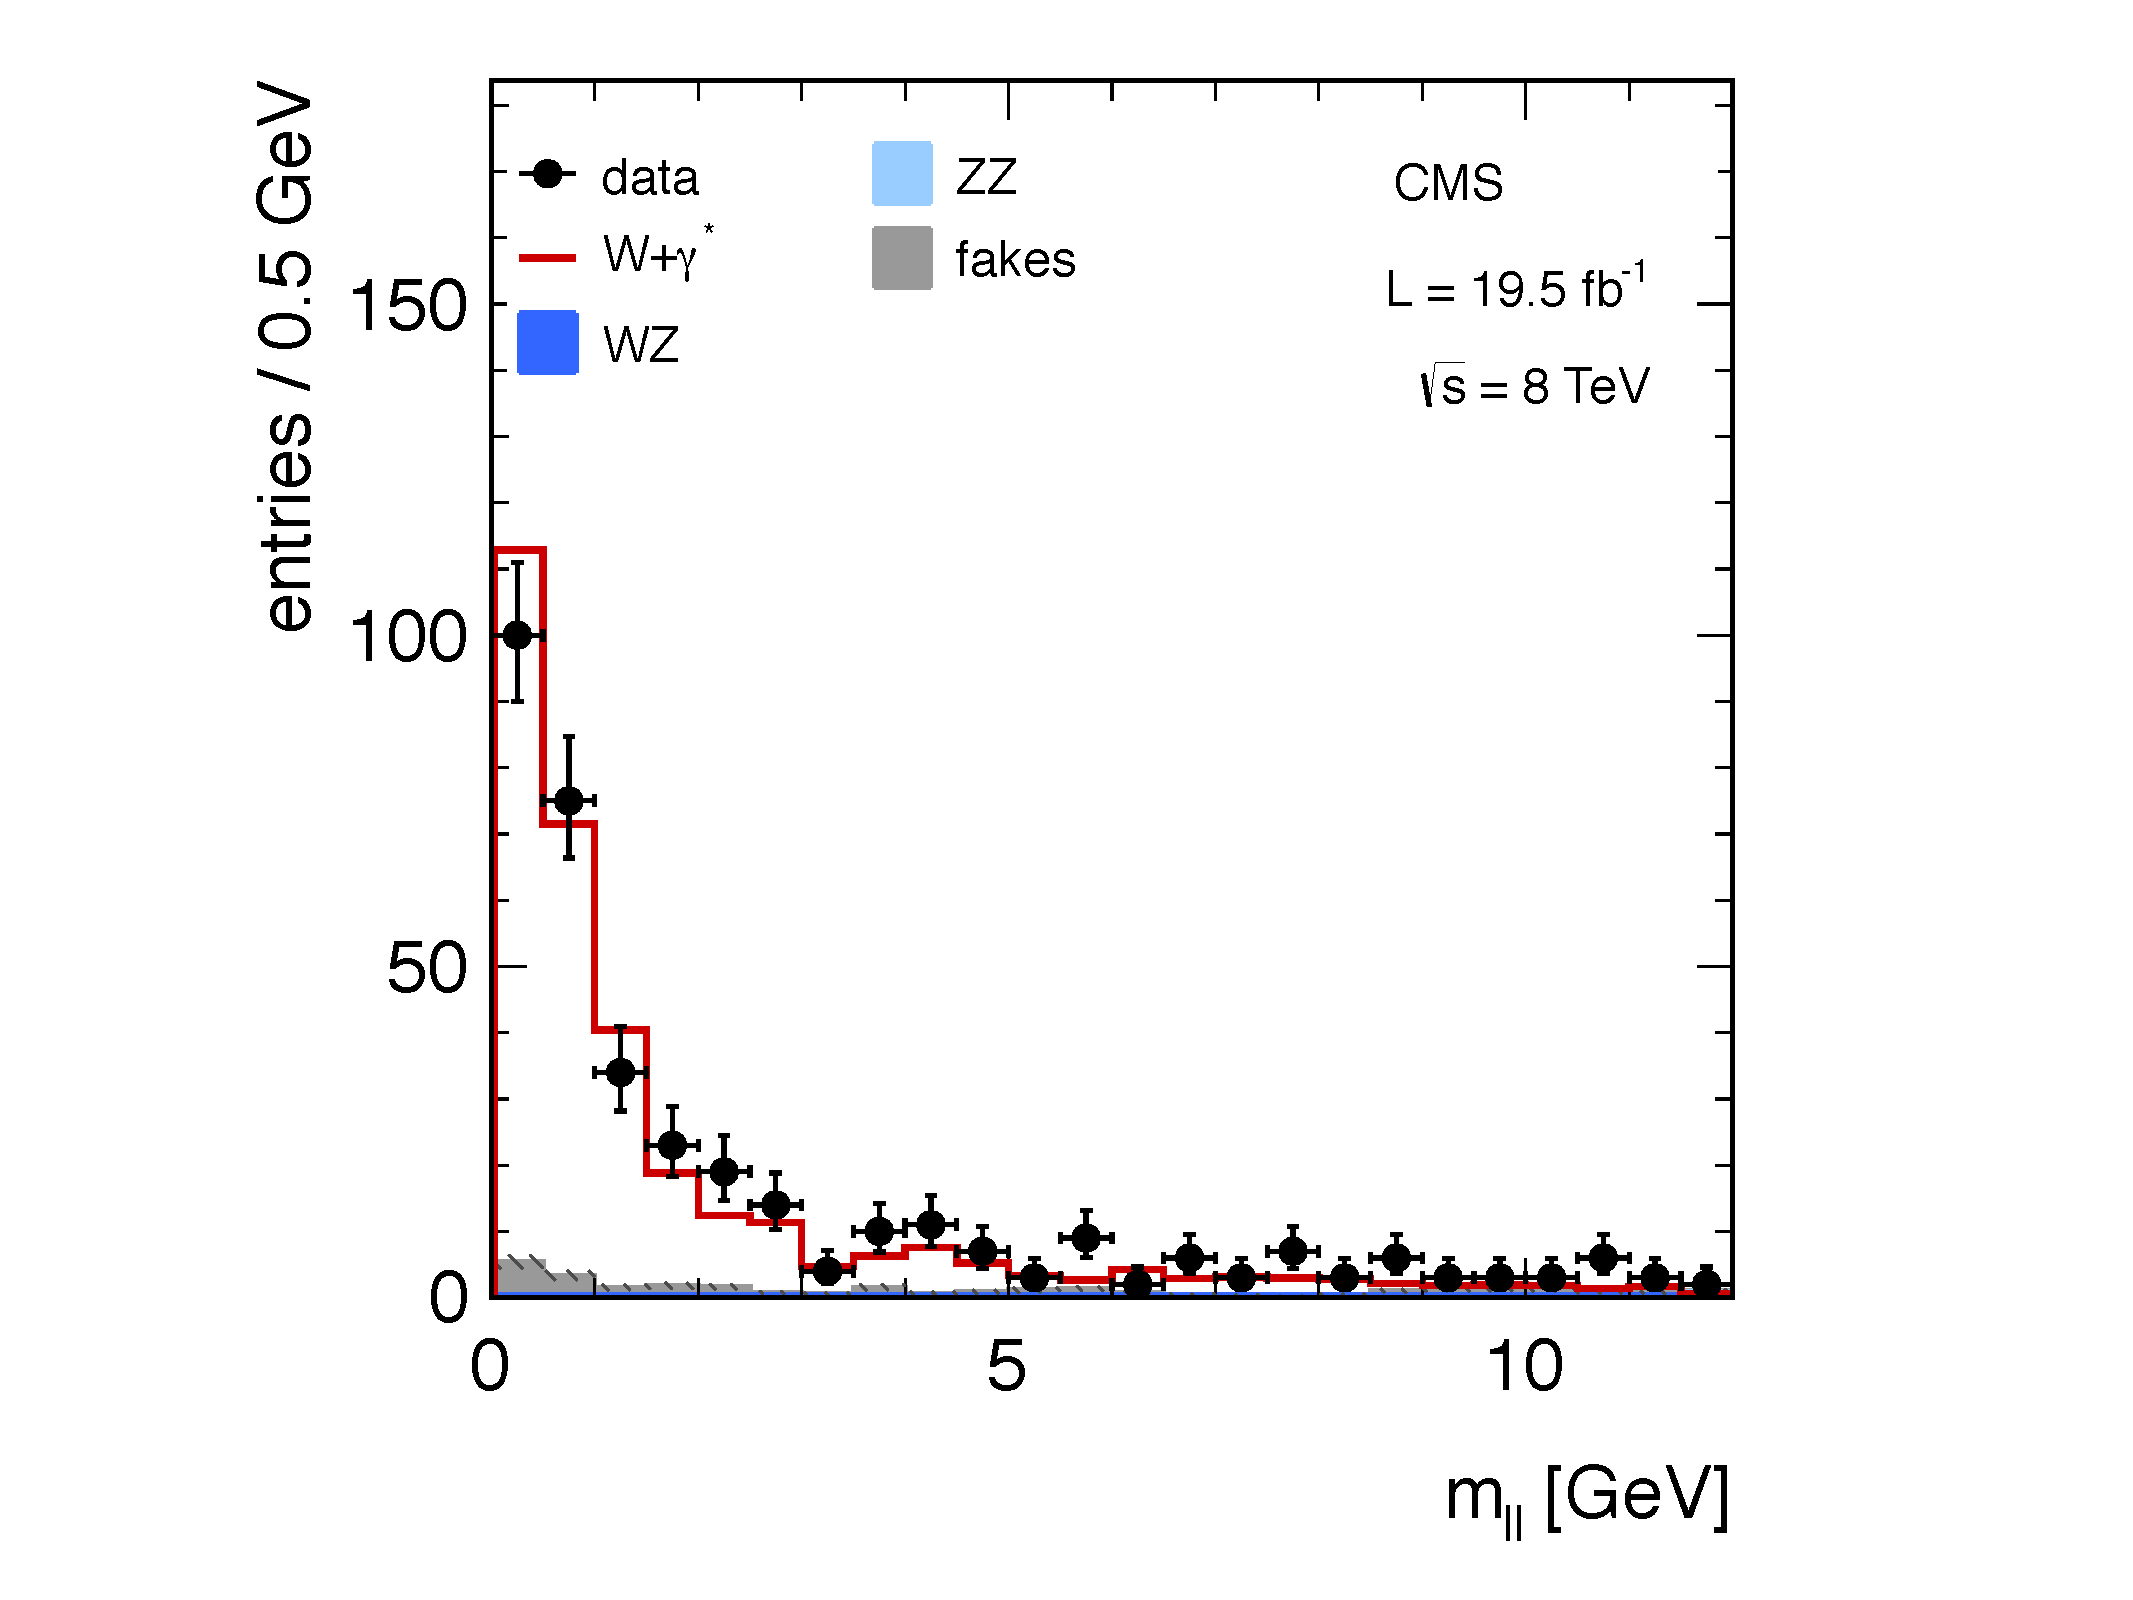
\includegraphics[width=0.8\textwidth]{figures/Wg3l.pdf} 
\end{tabular} 
\caption{\mll\ distribution for opposite-sign muon pairs after \wgammastar\ selection. 
The \wgammastar\ is normalized to match the data.} 
\label{fig:wg3l} 
\end{figure} 

%%%%%%%%%%%%%%%%%%%%%%%%%%
\section{ Other backgrounds } 

%%%%%
\subsection{\wgamma}

\wgamma\ can fake signal when the photon converts to a pair of electrons asymmetrically, 
giving a large fraction of its momentum to one of the electrons. 
This is difficult to be measured in data because it is hard to select 
events with asymmetric photon conversion due to fake electrons from \Wjets. 
So, we rely on simulation after data corrections such as trigger/lepton 
selection efficiencies and pileup.

For the shape-based method, the templates for \wgamma\ suffer from low statistics 
if the full lepton selection is applied to both leptons. So, we take the shape of the 
templates from \wgamma\ events before the photon converts to leptons, and apply 
photon-to-electron conversion probability($P(\gamma \rightarrow e)$) as a function of \Eta. 
The conversion 
factor is measured in simulation and shown in Figure~\ref{fig:photon_electron_ratio}.  
The function is parametrized with \Eta\ because conversion probability has strong 
correlation with the amount of material that the photon goes through.
\begin{figure}[htp] 
\centering 
\begin{tabular}{c} 
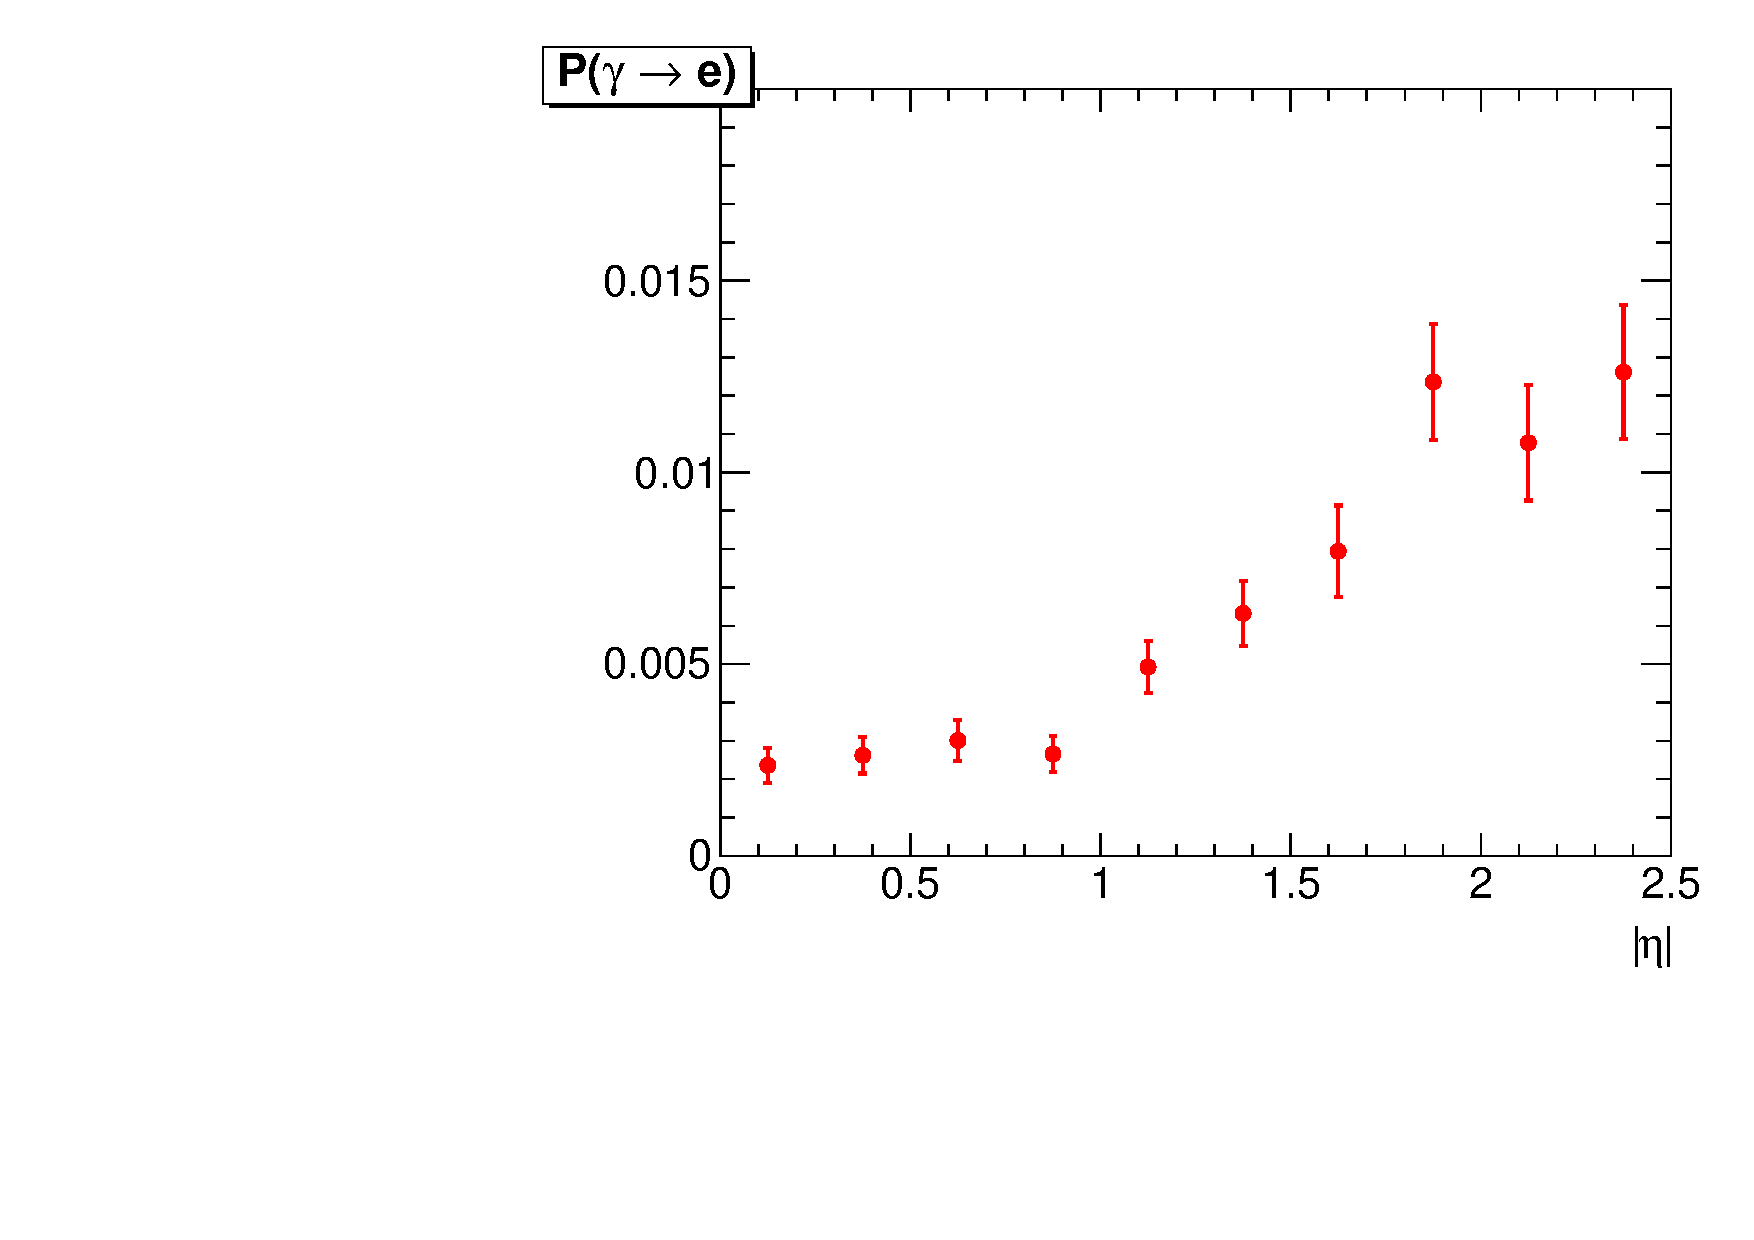
\includegraphics[width=0.7\textwidth]{figures/ratio_photon_electron.pdf} 
\end{tabular} 
\caption{The probability for a photon to convert to a pair of electrons, 
and one of the electrons is selected as a good electron.  } 
\label{fig:photon_electron_ratio} 
\end{figure}  

Figure~\ref{fig:wgamma_compare} shows the normalized \mll\ and \mT\ distributions 
of \wgamma\ samples, the red is the sample with 2 leptons in the final state 
and black is the sample with 1 lepton + $\gamma$ where the conversion 
factor is applied. The two shapes look consistent. 
By using the 1 lepton + $\gamma$ sample, we get an order of $\mathcal{O}(10^2)$ 
more statistics in the template.  
\begin{figure}[htp] 
\centering 
\begin{tabular}{c} 
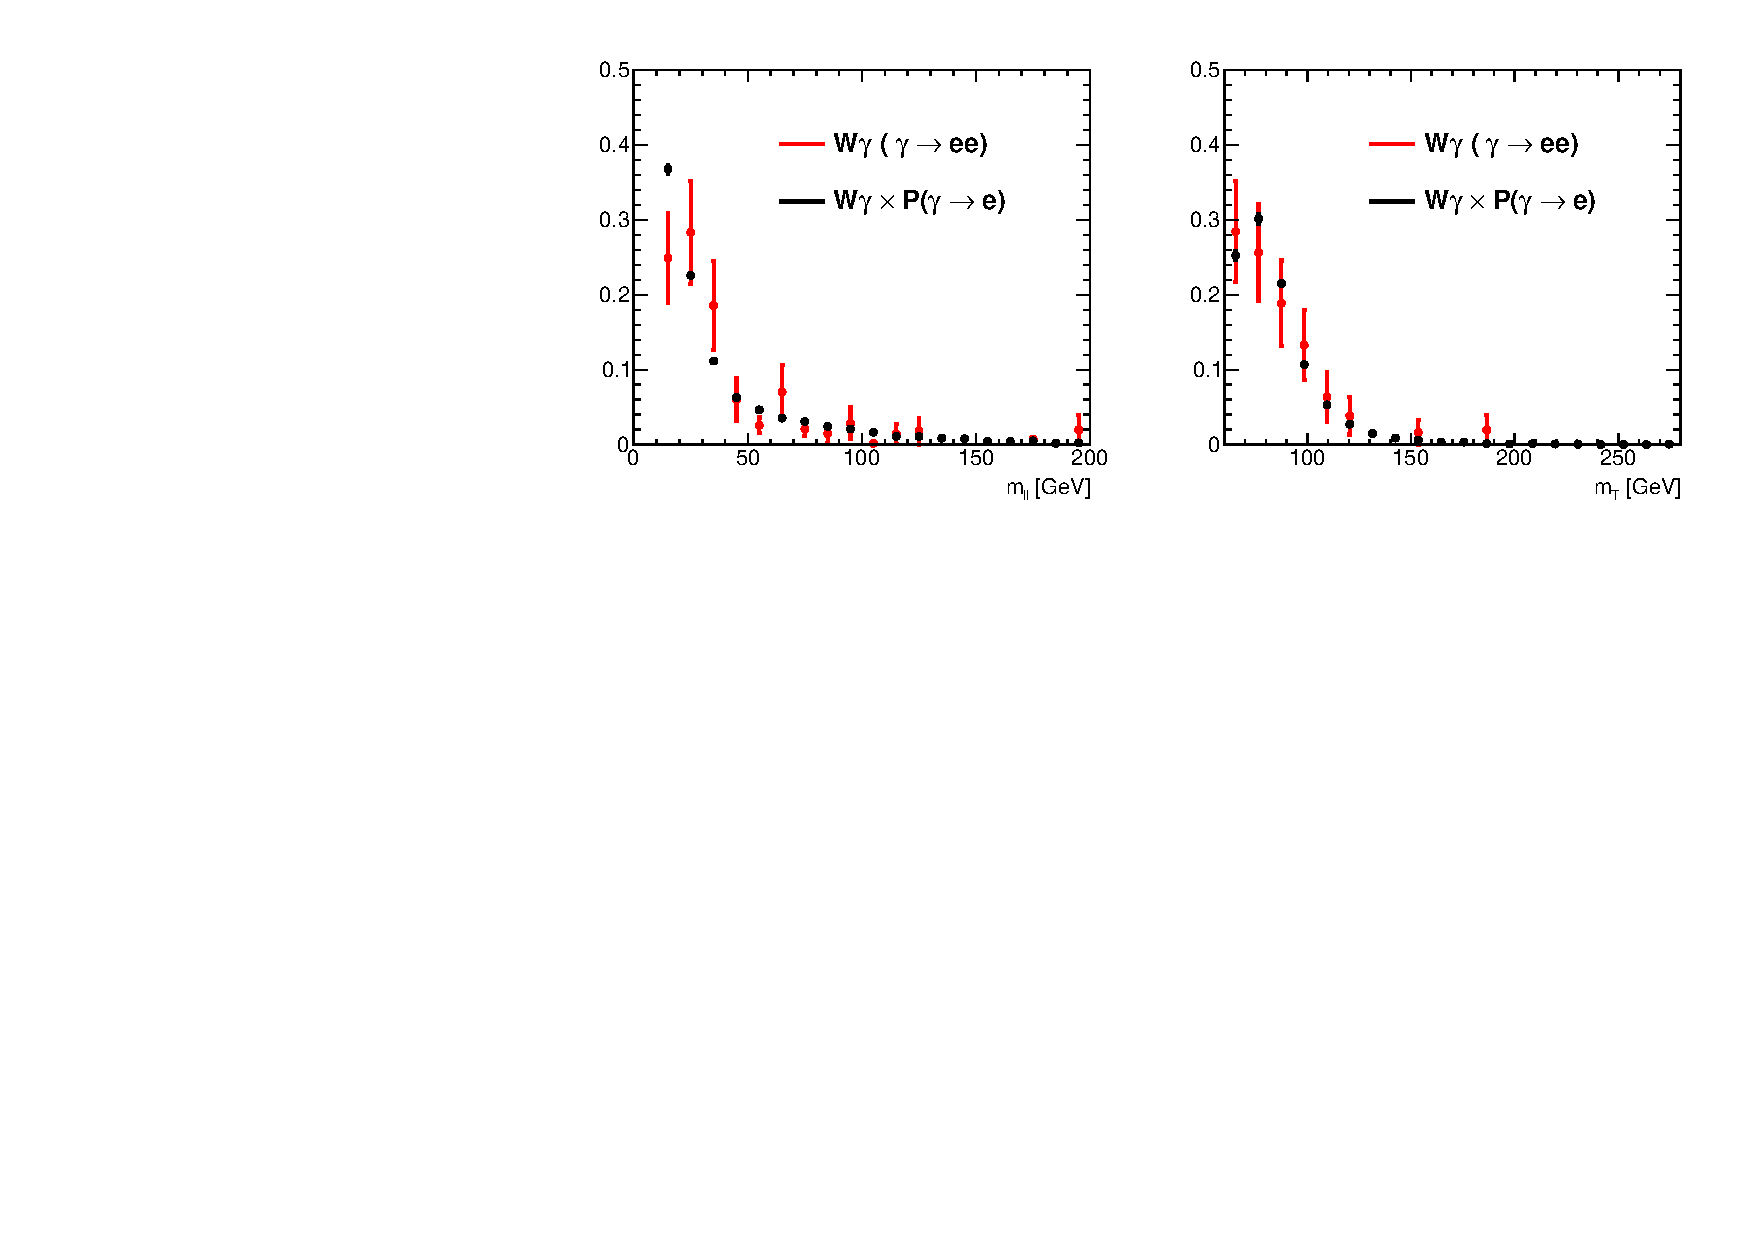
\includegraphics[width=1.0\textwidth]{figures/Wgamma_0j_of.pdf} 
\end{tabular} 
\caption{\mll\ and \mT\ distributions of \wgamma\ samples. 
Red is after photon coverts to electrons and black is before the photon conversion 
with the conversion probability applied. }
\label{fig:wgamma_compare} 
\end{figure}  



%%%%%
\subsection{\ztt}

The \ztt\ background contributes in the \DF\ category in case where 
the taus decay to $e$ or $\mu$ and neutrinos. 
In the \SF\ category, it is negligible thanks to \pmet\ which is 
designed to reduce \ztt\ background. 
Typically, the natural source 
of \met\ in \ztt\ gives soft \met, and a modest \met\ selection can  
reduce this background. But, in the environment of large number of pileup, 
the instrumental contribution to \met\ becomes larger, and it leads to large 
\met\ values. The cross section of the \ztt\ process is large, so we need to make 
sure that this background is under control. The simulation does not reproduce 
the instrumental \met\ properly, and we need a data-driven method to 
accurately estimate the \ztt\ background. 

The data-driven method for the estimation of \ztt\ background is done by the 
``tau embedding" technique~\cite{Chatrchyan:2014nva}. 
In this method, we select \dymm\ events in data
from the whole run range, 
and replace each muon with a simulated tau decay, 
$\tau \rightarrow l\bar{\nu}_l\nu_\tau$~\cite{Jadach:1990mz}. 
Then, the \met\ is re-calculated adding the neutrinos from the tau decays. 
Advantage of this method is that the event environment is taken from the real data, 
and the modeling of pileup, UE, jets and thus \met\ can be done consistently 
with real data. This sample is normalized to the inclusive \ztt\ MC 
at the level of requiring two leptons with lepton efficiency correction
and the branching fraction.

A 10 \% of systematic uncertainty of the method is assigned based on the MC closure test. 

%%%%%
\subsection{\vv} 

\vv\ backgrounds where the bosons decay leptonically are well-modelled by simulation.
In addition, the contribution of these backgrounds is small. Therefore, to estimate these 
background, we rely on simulation after data corrections 
such as trigger/lepton selection efficiencies and pileup.  



%%%%%%%%%%%%%%%%%%%%%%%%%%
\section{ The result of background estimation }

Table~\ref{tab:wwselection_all} summarizes the result of background estimation. 
It shows the yield of each process in the four final states, 0-jet \SF, 0-jet \DF,  
1-jet \SF\ and 1-jet \DF. Data and the total background yields are in good agreement. 
Actually, they should agree by design because backgrounds are normalized to data
by data-driven estimation. 

For comparison, Table~\ref{tab:cutbasedtable} shows the yields with $\mHi=125~\GeV$ Higgs 
selection shown in Table~\ref{tab:cutbasedtable}. The equivalent tables for other \mHi\ and 
7~\TeV\ are Table~\ref{tab:cut8tev} and \ref{tab:cut7tev}, respectively. 
After Higgs selection we see that data is in better agreement with prediction 
when Higgs signal at \mHi=125~\GeV\ is added. 

\begin{table}[ht!]
\begin{center}
\small
\vspace{0.5cm}
  \caption{Expected number of signal and background events from the data-driven methods for 
  at 8~\TeV\ after applying \WW\ selection. 
  Only statistical uncertainties are reported.}
\label{tab:wwselection_all}
\vspace{0.5cm}
\begin{tabular}{c|c|c|c|c}
\hline
                & \multicolumn{2}{c|}{0-jet}             &          \multicolumn{2}{c}{1-jet}             \\
\hline
                &  \SF                &   \DF             &           \SF     &  \DF               \\
\hline \hline
\qqww           & 1782.4 $\pm$ 11.6        & 4402.1 $\pm$ 18.0 &  533.7 $\pm$  6.0  &  1414.3 $\pm$   9.7 \\
\ggww           &  124.0 $\pm$  2.2        &  223.7 $\pm$  3.0 &        34.1 $\pm$  1.1  &    76.3 $\pm$   1.6 \\
\topbkg         &  273.3 $\pm$  7.8        &  563.7 $\pm$ 11.1 &  677.2 $\pm$ 10.4  &  1644.2 $\pm$  16.8  \\
\wgamma         &   23.5 $\pm$  5.7        &  140.0 $\pm$ 16.9 &        11.9 $\pm$  4.8  &    51.8 $\pm$   9.2 \\
\wgammastar     &   13.7 $\pm$  2.0        &  147.9 $\pm$  6.5 &         2.4 $\pm$  0.8  &    23.9 $\pm$   2.7 \\
%VVV             &   19.8 $\pm$  1.0        &   38.3 $\pm$  1.4 &        16.3 $\pm$  1.5  &    33.4 $\pm$   1.7 \\
%\vv              &   36.8 $\pm$  0.6        &  105.5 $\pm$  1.0 &        23.4 $\pm$  0.5  &   100.7 $\pm$   1.0 \\
\vv              &  56.6 $\pm$  1.2        &  143.8 $\pm$  1.7 &        39.7 $\pm$  1.6  &   134.1 $\pm$   2.0 \\
$\Wjets$        &  107.5 $\pm$  4.6        &  694.8 $\pm$ 10.3 &        47.4 $\pm$  3.6  &   356.2 $\pm$   7.9 \\
$\Zjets$        &  294.6 $\pm$ 60.3        &   82.5 $\pm$  1.4 &  118.4 $\pm$ 30.3  &   248.7 $\pm$   2.8  \\
\hline \hline
Total Background      & 2676.3 $\pm$ 62.5     & 6399.1 $\pm$ 30.1 & 1465.3 $\pm$ 33.3 &   3950.0 $\pm$  23.7   \\
\hline
\ggH        &  $83.87\pm1.63$   & $237.24\pm2.67$ & $25.68\pm0.91$  & $94.97\pm1.71$  \\
\qqH        &  $0.87\pm0.05$   & $3.08\pm0.09$ & $3.78\pm0.09$  & $12.4\pm0.17$  \\
\hline \hline
Data            & 2728                  & 6361                & 1477             & 3944    \\
\hline
\end{tabular}
\end{center}
\end{table}
%
\begin{table}[ht!]
\begin{center}
\small
\vspace{0.5cm}
  \caption{Expected number of signal and background events from the data-driven methods for 
  at 8~\TeV\ after applying $\mHi=125~\GeV$ Higgs selection shown in 
  Table~\ref{tab:cutbasedtable}. Total uncertainties(statistical$\oplus$systematic) 
  are reported.}
\label{tab:wwselection_all}
\vspace{0.5cm}
\begin{tabular}{c|c|c|c|c}
\hline
                & \multicolumn{2}{c|}{0-jet}             &          \multicolumn{2}{c}{1-jet}             \\
\hline
                &  \SF                &   \DF             &           \SF     &  \DF               \\
\hline \hline
\qqww       &     $197.2\pm19.2$ & $294.1\pm28.4$ & $37.5\pm5.3$ & $74.5\pm10.4$ \\
\ggww       & $9.7\pm3.1$   & $16.0\pm5.0$  & $2.2\pm0.8$   & $4.8\pm1.6$ \\
\topbkg     & $9.3\pm2.2$   & $20.0\pm4.3$  & $40.4\pm3.1$  & $78.8\pm4.5$ \\
\wgamma     & $3.2\pm2.5$   & $21.2\pm9.8$  & $2.5\pm1.5$   & $6.8\pm4.0$ \\
\wgammastar & $6.1\pm2.9$   & $18.3\pm8.1$  & $0.8\pm0.7$   & $4.5\pm2.3$ \\
\vv         & $13.3\pm1.3$  & $10.2\pm1.0$  & $6.5\pm1.0$   & $10.2\pm1.1$  \\
%\WjetsE     & $12.1\pm4.5$  & $26.4\pm9.6$  & $2.8\pm1.2$   & $12.7\pm4.7$ \\
%\WjetsM     & $16.5\pm6.2$  & $21.4\pm8.0$  & $3.7\pm1.6$   & $12.9\pm5.0$ \\
\Wjets      & $28.6\pm10.7$ & $47.8\pm17.6$ & $6.5\pm2.8$   & $25.6\pm9.7$ \\
\Zjets      & $92.2\pm31.0$ & $1.2\pm0.2$   & $14.7\pm5.3$  & $2.7\pm0.4$ \\
\hline \hline
Total Background    & $359.6\pm37.6$    & $428.8\pm34.2$    & $111.0\pm8.6$ & $208.0\pm14.1$ \\
\hline
\ggH        &     $55.8\pm12.2$   & $88.9\pm19.3$ & $15.9\pm5.2$  & $37.5\pm12.2$  \\
\qqH        &     $0.5\pm0.1$     &  $1.0\pm0.1$  & $2.1\pm0.2$   &   $4.6\pm0.5$  \\ 
\hline \hline
Data                & 421               & 505               & 140           & 228 \\
\hline
\end{tabular}
\end{center}
\end{table}
